\chapter{THỰC NGHIỆM VÀ ĐÁNH GIÁ KẾT QUẢ}
\label{chap:chapter4}

\section{Cấu hình thực nghiệm}
\label{sec:cauHinh}

\subsection{Môi trường phần cứng và phần mềm}
\label{subsec:phanCung}

Môi trường thực nghiệm được triển khai trên nền tảng Python với các thư viện
cốt lõi: PyTorch (cài đặt mạng Actor--Critic và thuật toán PPO), Gymnasium
\parencite{towers2024gymnasium} (giao diện môi trường mô phỏng), NumPy và
Pandas (xử lý dữ liệu M5 và tính toán thống kê), SciPy (kiểm định thống kê).

Quá trình huấn luyện của đợt thực nghiệm cuối chạy trên một GPU NVIDIA GeForce
RTX 3050 Laptop (PyTorch, CUDA); phần mô phỏng môi trường vector hóa và các
chính sách cổ điển chạy trên CPU. Kết quả báo cáo trong chương này dựa trên $3$
lần huấn luyện độc lập (Mục~\ref{subsec:daHatGiong}), mỗi lần $10.000$
episode, mất lần lượt $280$, $243$ và $219$ phút (hạt giống $42$, $1$, $2$),
tổng cộng khoảng $12{,}4$ giờ. Mỗi thí nghiệm loại trừ $1.000$ episode mất
khoảng $22$--$34$ phút. Khóa luận không đối chiếu thời gian huấn luyện với các
công trình khác, vì khác bài toán, phần cứng và quy mô nên đó không phải là bằng
chứng so sánh.

\subsection{Nguồn dữ liệu và tiền xử lý}
\label{subsec:duLieu}

Khóa luận sử dụng hai tệp chính từ bộ dữ liệu M5
\parencite{makridakis2022background, m5dataset}:
\path{sales_train_evaluation.csv} chứa $30.490$ chuỗi doanh số theo ngày
($3.049$ mặt hàng $\times$ $10$ cửa hàng) trên $1.941$ ngày, và
\path{calendar.csv} chứa thông tin lịch, ngày lễ và các sự kiện trợ cấp thực
phẩm SNAP.

Quy trình sàng lọc mặt hàng. Không phải mọi tổ hợp cửa hàng --- mặt
hàng đều tạo thành một bài toán đặt hàng lại. Trong bộ dữ liệu gốc có một tỷ lệ
đáng kể các cặp mà cửa hàng trên thực tế không kinh doanh mặt hàng đó, thể hiện
qua chuỗi doanh số gần như bằng không suốt toàn bộ giai đoạn. Đưa những chuỗi
này vào tập huấn luyện không làm bài toán khó hơn mà chỉ bổ sung nhiễu vào
gradient của mạng dùng chung. Khóa luận vì vậy chỉ giữ lại các mặt hàng có nhu
cầu trung bình từ $0{,}2$ đơn vị mỗi ngày trở lên tại ít nhất $80\%$ số cửa
hàng, tính trên miền huấn luyện. Từ $3.049$ mặt hàng ban đầu, $1.762$ mặt hàng
vượt ngưỡng; trong số đó $M = 30$ mặt hàng được chọn theo phương pháp phân tầng
trên ba nhóm ngành hàng (Foods, Hobbies, Household) nhằm bảo đảm dải quy mô nhu
cầu trải rộng.

Bảng~\ref{tab:dacTrungDuLieu} so sánh đặc trưng của tập thực nghiệm với bộ dữ
liệu gốc. Điểm cần lưu ý là tỷ lệ ngày không phát sinh giao dịch vẫn ở mức
$57{,}4\%$: quy trình sàng lọc loại bỏ các chuỗi thoái hóa nhưng không
làm mất đi tính gián đoạn --- vốn là đặc trưng khiến bài toán trở nên khó và là
một trong những lập luận nền của khóa luận.

\begin{table}[htbp]
    \centering
    \caption{Đặc trưng nhu cầu của tập thực nghiệm so với bộ dữ liệu gốc}
    \label{tab:dacTrungDuLieu}
    \begin{tabular}{|l|c|c|}
        \hline
        \textbf{Chỉ tiêu} & \textbf{M5 gốc} & \textbf{Tập thực nghiệm} \\
        \hline
        Số chuỗi (cặp kho--mặt hàng) & $30.490$ & $300$ \\ \hline
        Nhu cầu trung bình (đv/ngày) & $1{,}13$ & $3{,}24$ \\ \hline
        Trung vị nhu cầu (đv/ngày)   & $0{,}45$ & $0{,}74$ \\ \hline
        Tỷ lệ ngày bằng không        & $68{,}0\%$ & $57{,}4\%$ \\ \hline
        Cặp có nhu cầu $< 0{,}1$ đv/ngày & --- & $5/300$ \\
        \hline
    \end{tabular}
\end{table}

Tách miền thời gian. Chuỗi $1.941$ ngày được chia theo trục thời gian thành ba
miền không chồng lấn, mỗi miền có một vai trò cố định
(Bảng~\ref{tab:baMien}). Mọi đại lượng ước lượng từ dữ liệu --- nhu cầu trung
bình $\bar{D}^{(i)}$ dùng cho bảng mức đặt hàng, sức chứa kho, mẫu số chuẩn hóa
phần thưởng --- chỉ lấy từ miền huấn luyện. Miền kiểm tra không được dùng để
chọn mô hình, chỉnh phần thưởng hay tinh chỉnh baseline.

\begin{table}[htbp]
    \centering
    \caption{Ba miền dữ liệu và vai trò của từng miền}
    \label{tab:baMien}
    \small
    \resizebox{\textwidth}{!}{%
\begin{tabular}{llcp{6.2cm}}
        \toprule
        \textbf{Miền} & \textbf{Chỉ số ngày} & \textbf{Ngày lịch (số ngày)} & \textbf{Được phép dùng để} \\
        \midrule
        Huấn luyện & $[0,\ 1050)$ & 29/01/2011--13/12/2013 ($1.050$) & Thu rollout và cập nhật PPO; ước lượng $\bar{D}^{(i)}$, sức chứa kho, mẫu số chuẩn hóa \\
        Validation & $[1050,\ 1450)$ & 14/12/2013--17/01/2015 ($400$) & Chọn checkpoint IPPO; tinh chỉnh tham số baseline; so sánh các cấu hình huấn luyện \\
        Kiểm tra (test) & $[1450,\ 1941)$ & 18/01/2015--22/05/2016 ($491$) & \emph{Chỉ} báo cáo kết quả cuối; không dùng cho bất kỳ quyết định thiết kế nào \\
        \bottomrule
    \end{tabular}}
\end{table}

Ngày $0$ là dòng đầu tiên của \path{calendar.csv} (29/01/2011). Các cửa sổ thời
gian đặc trưng của mô hình gồm: lịch sử nhu cầu $w = 7$ ngày trong vector quan
sát, fill rate trên cửa sổ trượt $30$ ngày, mỗi episode huấn luyện dài $365$ ngày
cắt từ miền huấn luyện, và mỗi lần đánh giá chạy trọn $491$ ngày của miền test.
Cú sốc cầu nhân tạo ở Mục~\ref{subsec:hanChe} bắt đầu ở ngày $1650$ (06/08/2015)
và kéo dài $28$ ngày, tức nằm trong miền test.

\subsection{Thiết lập kịch bản mô phỏng}
\label{subsec:kichBan}

\begin{table}[htbp]
    \centering
    \caption{Cấu hình môi trường mô phỏng}
    \label{tab:cauHinhEnv}
    \begin{tabular}{|l|c|}
        \hline
        \textbf{Tham số} & \textbf{Giá trị} \\
        \hline
        Số kho ($N$) & $10$ \\ \hline
        Số mặt hàng ($M$) & $30$ \\ \hline
        Số tác tử ($N \times M$) & $300$ \\ \hline
        Độ dài episode & $365$ ngày \\ \hline
        Cửa sổ nhìn lại ($w$) & $7$ ngày \\ \hline
        Lead time & $\text{Uniform}\{1, 2, 3\}$ ngày \\ \hline
        Bội số mức đặt hàng ($\mathbf{m}$) & $\{0;\,0{,}5;\,1;\,2;\,3;\,5\}$ \\ \hline
        Sức chứa kho ($\kappa$) & $5{,}0$ ngày nhu cầu của từng kho \\ \hline
        Ngưỡng fill rate ($\tau$) & $85\%$ \\
        \hline
    \end{tabular}
\end{table}

Lựa chọn $\kappa = 5{,}0$ được xác định bằng thực nghiệm. Với
$\kappa = 3{,}0$, mức phục vụ cao nhất mà bất kỳ chính sách nào đạt được chỉ là
$79{,}5\%$ --- mục tiêu $85\%$ trở thành bất khả thi. Với $\kappa \ge 12{,}0$,
chi phí tràn kho bằng không: ràng buộc không còn hiệu lực và bài toán suy biến
thành $300$ bài toán độc lập, mất đi bản chất đa tác tử. Tại $\kappa = 5{,}0$,
mục tiêu $85\%$ khả thi trong khi chi phí tràn kho vẫn chiếm khoảng
$1$--$2\%$ tổng chi phí, nghĩa là ràng buộc thực sự có hiệu lực.

\section{Phương pháp đối chứng}
\label{sec:baselines}

Hiệu năng của IPPO được so sánh với ba chính sách tồn kho cổ điển: EOQ
\cite{harris1913}, $(s, S)$ \cite{scarf1960} và Newsvendor \cite{arrow1951}.

Điều kiện so sánh công bằng. Ba yếu tố được kiểm soát. Thứ nhất,
tham số của cả ba chính sách được tối ưu bằng tìm kiếm lưới trên chính môi
trường mô phỏng, ở \emph{miền validation}, theo \emph{cùng tiêu chí} dùng để
chọn checkpoint IPPO: chi phí vận hành thấp nhất trong số các cấu hình đạt fill
rate $\ge 85\%$; nếu không cấu hình nào đạt, chọn cấu hình có fill rate cao
nhất. Thứ hai, các chính sách cổ điển truy cập cùng một tập thông tin với tác tử
IPPO: nhu cầu trung bình và độ lệch chuẩn ước lượng từ miền huấn luyện, cùng
lịch sử nhu cầu gần nhất. Thứ ba, cả bốn phương pháp chịu cùng ràng buộc rời rạc
hóa: lượng đặt hàng mong muốn được làm tròn về mức gần nhất trong sáu mức của
công thức (\ref{eq:orderTable}).

Mỗi chính sách cổ điển được đánh giá ở hai phiên bản. Phiên bản thứ nhất dùng
\emph{một bộ tham số chung} cho cả $300$ cặp. Phiên bản thứ hai dùng \emph{một bộ
tham số riêng cho mỗi nhóm quy mô nhu cầu} (bốn nhóm: dưới $0{,}5$; $0{,}5$--$2$;
$2$--$10$; từ $10$ đơn vị mỗi ngày trở lên), được tìm bằng tìm kiếm theo tọa độ:
xuất phát từ bộ tham số chung, lần lượt tối ưu tham số của từng nhóm trong khi
giữ nguyên các nhóm khác, với cùng tiêu chí chi phí thấp nhất trong số cấu hình
đạt fill rate $\ge 85\%$. Phiên bản theo nhóm là đối thủ mạnh hơn và sát với cách
doanh nghiệp đặt chính sách theo nhóm hàng; nó được đưa vào để tránh so sánh IPPO
--- vốn điều chỉnh theo trạng thái của từng cặp --- với một đối thủ bị giới hạn ở
một bộ tham số duy nhất.

Ràng buộc thứ ba được giữ cho mọi phương pháp vì nó mô phỏng một ràng buộc vận
hành chung: đơn bổ sung hàng được đặt theo một số lô chuẩn tỷ lệ với nhu cầu
trung bình của mặt hàng, chứ không theo số lượng tùy ý. Nếu chỉ IPPO bị giới
hạn ở sáu mức còn baseline được đặt số lượng liên tục, hai bên sẽ khác nhau cả
về không gian hành động lẫn thuật toán, và so sánh không còn cô lập được tác
động của thuật toán. Hệ quả là các baseline có thể kém hơn phiên bản đặt số
lượng tùy ý của chúng; khóa luận ghi nhận đây là một giới hạn của phép so sánh
(Mục~\ref{sec:hanCheChuong4}).

Bảng~\ref{tab:thamSoBaseline} liệt kê tham số tối ưu tìm được.

\begin{table}[htbp]
    \centering
    \caption{Tham số tối ưu của các chính sách đối chứng (một bộ tham số chung
    cho $300$ cặp), tìm kiếm lưới trên miền validation}
    \label{tab:thamSoBaseline}
    \begin{tabular}{|l|l|}
        \hline
        \textbf{Chính sách} & \textbf{Tham số tối ưu} \\
        \hline
        EOQ        & $q_{\text{factor}} = 3{,}0$; $L = 4{,}0$ \\ \hline
        $(s, S)$   & $\alpha = 0{,}70$; $q_{\text{factor}} = 1{,}0$; $L = 3{,}0$ \\ \hline
        Newsvendor & $CR = 0{,}60$; $L = 4{,}0$ \\
        \hline
    \end{tabular}
\end{table}

Ở phiên bản theo nhóm, bộ tham số thay đổi theo quy mô nhu cầu; chẳng hạn
$q_{\text{factor}}$ của EOQ tăng từ $1{,}0$ (nhóm dưới $0{,}5$ đơn vị mỗi ngày)
lên $3{,}0$ (nhóm từ $10$ đơn vị mỗi ngày trở lên), và $CR$ của Newsvendor là
$0{,}60$; $0{,}75$; $0{,}85$; $0{,}60$ lần lượt theo bốn nhóm. Cả ba chính sách
theo nhóm đều đạt fill rate trên miền validation sát ngưỡng $85\%$
($85{,}0$--$85{,}3\%$), tức tiêu chí chọn cấu hình rẻ nhất đẩy các baseline về
sát biên ràng buộc.

Một quan sát đáng chú ý: tỷ số tới hạn lý thuyết của mô hình Newsvendor với bộ
tham số chi phí đang dùng là $c_{th}/(c_{th} + c_{lk}) = 10/11 \approx 0{,}909$,
nhưng tìm kiếm lưới trên miền validation cho $CR = 0{,}60$ --- thấp hơn nhiều.
Chênh lệch này không xuất phát từ sai lệch triển khai mà phản ánh hai khác biệt.
Thứ nhất, tỷ số tới hạn cổ điển tối ưu cho \textit{mức phục vụ chu kỳ} $\alpha$
trong bài toán một kỳ không có hàng đang về, trong khi môi trường ở đây là nhiều
kỳ, có lượng hàng trên đường vận chuyển và ràng buộc sức chứa. Thứ hai, tiêu chí
chọn tham số là chi phí vận hành thấp nhất trong số cấu hình đạt fill rate $\ge
85\%$, chứ không phải mức phục vụ cao nhất. Kết quả này phù hợp với nhận định của
Zipkin \cite{zipkin2008} rằng các chính sách cổ điển không còn tối ưu đã được
chứng minh trong bối cảnh mất đơn hàng.

\section{Giao thức đánh giá}
\label{sec:giaoThuc}

\subsection{Quy trình đánh giá}
\label{subsec:daHatGiong}

Chính sách IPPO được đánh giá ở chế độ tất định (chọn hành động có xác suất cao
nhất) trên \emph{toàn bộ quỹ đạo kiểm tra}: một lần chạy đi qua trọn $491$ ngày
của miền test ($[1450,\ 1941)$), với chuỗi nhu cầu cố định là nhu cầu thực tế
của M5. Nguồn ngẫu nhiên duy nhất còn lại là thời gian giao hàng; lần chạy được
lặp lại với $30$ hạt giống ngẫu nhiên của thời gian giao hàng. Mọi chính sách
chạy trên đúng cùng $30$ hạt giống, nên mỗi hạt giống $j$ cho một cặp quan sát
$(C_j^{\text{IPPO}}, C_j^{\text{baseline}})$. Cách làm này thay cho giao thức cũ
dùng $30$ cửa sổ $365$ ngày cắt từ một miền chỉ dài $491$ ngày --- các cửa sổ đó
chồng lấn mạnh với nhau nên không thể coi là $30$ quan sát độc lập.

Kiểm định thống kê được thực hiện trên hiệu số theo cặp
$\Delta C_j = C_j^{\text{IPPO}} - C_j^{\text{baseline}}$: báo cáo hiệu trung
bình kèm khoảng tin cậy $95\%$, kiểm định $t$ theo cặp, kiểm định hạng có dấu
Wilcoxon và hệ số ảnh hưởng theo cặp $d_z = \overline{\Delta C} / s_{\Delta C}$.
Các lần đánh giá của IPPO ở những hạt giống huấn luyện khác nhau không được gộp
chung với các lần đánh giá baseline như những quan sát độc lập.

Theo khuyến nghị của Henderson và cộng sự \cite{henderson2018} và Agarwal và
cộng sự \cite{agarwal2021} về việc không nên suy luận từ một lần huấn luyện
duy nhất, IPPO được huấn luyện độc lập trên $3$ hạt giống huấn luyện
(\texttt{seed} $\in \{42, 1, 2\}$) với cùng ngân sách $10.000$ episode mỗi hạt
giống. Checkpoint của từng hạt giống được chọn trên miền validation theo tiêu
chí ở Mục~\ref{subsec:fillRate} (chi phí validation thấp nhất trong các lần đánh
giá đạt fill rate $\ge 85\%$; được chọn ở episode $3.775$, $4.950$ và $5.250$
tương ứng), rồi đánh giá riêng trên miền test theo quy trình
trên. Kết quả được báo cáo \emph{theo từng hạt giống} (mỗi hạt giống một kiểm
định theo cặp), sau đó tổng hợp bằng trung bình và độ lệch chuẩn \emph{giữa các
hạt giống}, cùng số hạt giống cho kết luận có ý nghĩa thống kê. Mọi thí nghiệm
loại trừ (Mục~\ref{sec:phanTich}) dùng ngân sách $1.000$ episode, được so với
một lần chạy tham chiếu cùng hạt giống và cùng ngân sách, vì lịch giảm tốc độ
học và hệ số entropy phụ thuộc vào tổng số episode; các thí nghiệm về thiết kế
phần thưởng được lặp lại trên cả $3$ hạt giống, còn các thí nghiệm loại trừ khác
và thí nghiệm hold-out chỉ chạy một hạt giống ($42$).

\subsection{Các chỉ số đánh giá}
\label{subsec:chiSo}

\begin{enumerate}
    \item Tổng chi phí vận hành (công thức~\ref{eq:chiPhiVanHanh}): tổng
    bốn thành phần chi phí thực phát sinh (lưu kho, thiếu hàng, đặt hàng, tràn
    kho) trên toàn quỹ đạo kiểm tra và $300$ cặp. Thành phần phạt vi phạm mức phục vụ không được tính vào chỉ
    số này, vì nó là tín hiệu định hướng học chứ không phải chi phí kế toán.

    \item Tỷ lệ đáp ứng nhu cầu (fill rate $\beta$): tỷ số giữa tổng
    lượng hàng bán được và tổng nhu cầu phát sinh trên cả episode.

    \item Cơ cấu chi phí thành phần: dùng để nhận diện chiến lược mà
    mỗi phương pháp áp dụng.

    \item Đường cong học: phần thưởng, fill rate, entropy của chính
    sách và explained variance của Critic qua các episode huấn luyện.
\end{enumerate}

\section{Kết quả thực nghiệm}
\label{sec:ketQua}

\subsection{Quá trình huấn luyện và tính hội tụ}
\label{subsec:hoiTu}

Hình~\ref{fig:duongCongHoc} trình bày bốn chỉ số theo dõi quá trình huấn luyện
của hạt giống \texttt{seed}~$=42$, đại diện cho hình dạng đường cong học chung
của cả $3$ hạt giống (Mục~\ref{subsec:daHatGiong}).

\begin{figure}[htbp]
    \centering
    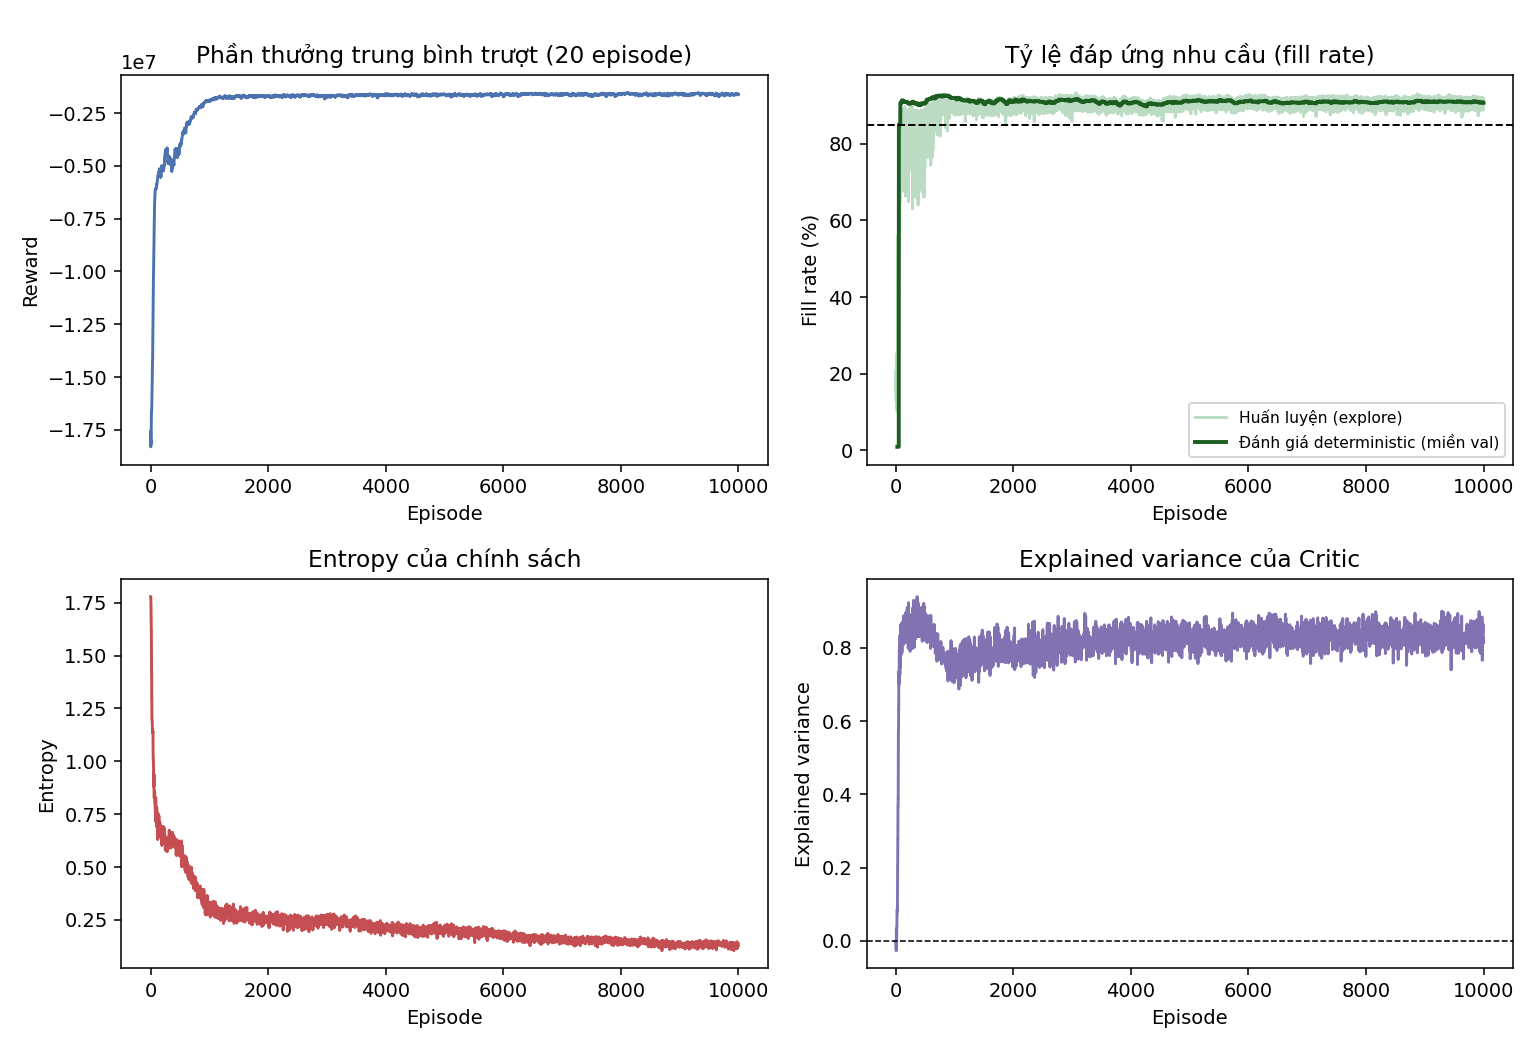
\includegraphics[width=\textwidth]{media/duong_cong_hoc.png}
    \caption{Diễn biến huấn luyện qua $10.000$ episode (hạt giống $42$): (a)
    phần thưởng tích lũy; (b) tỷ lệ đáp ứng nhu cầu; (c) entropy của chính
    sách; (d) explained variance của Critic}
    \label{fig:duongCongHoc}
\end{figure}

Phần thưởng tăng từ $-17{,}59$ triệu ở episode đầu lên quanh $-1{,}61$ triệu
(trung bình $200$ episode cuối, dao động trong khoảng $-2{,}25$ đến $-1{,}48$
triệu), tức giảm khoảng $91\%$ tổng chi phí so với chính sách khởi tạo ngẫu
nhiên. Phần thưởng làm mượt đi vào khoảng $5\%$ quanh giá trị cuối từ khoảng
episode $1.200$ và từ đó đi ngang: chi phí validation tốt nhất ở $20\%$ episode
cuối chỉ lệch $+1{,}6\%$ so với phần trước đó ở hạt giống $42$ ($+0{,}2\%$ và
$+1{,}3\%$ ở hai hạt giống còn lại), nên huấn luyện dài hơn $10.000$ episode
không còn cải thiện đáng kể. Đường cong không sụp đổ sau điểm hội tụ --- đặc
tính mong đợi của cơ chế mục tiêu bị chặn (clipped objective) trong PPO.

Hai chỉ số còn lại xác nhận rằng cả hai nửa của thuật toán đều thực sự học.
Entropy của chính sách giảm từ $1{,}779$ --- gần đúng giá trị $\ln 6 = 1{,}792$
của phân phối đều trên sáu hành động --- xuống $0{,}138$ ở episode cuối ($0{,}128$
trung bình $100$ episode cuối), nghĩa là chính sách đã định hình rõ rệt thay vì
còn chọn ngẫu nhiên. Explained variance của Critic vượt $0{,}6$ sau khoảng $50$
episode đầu, sau đó dao động trong khoảng $0{,}69$--$0{,}94$ (trung bình $0{,}84$
ở $200$ episode cuối), nghĩa là hàm giá trị giải thích được phần lớn phương sai
của phần thưởng tích lũy thực tế. Độ lệch KL xấp xỉ ở episode cuối là
$2{,}4 \times 10^{-4}$, nằm sâu dưới ngưỡng $0{,}02$, cho thấy chính sách đã ổn
định chứ không còn dao động mạnh giữa các lần cập nhật.

Tỷ lệ đáp ứng khi huấn luyện vượt ngưỡng mục tiêu $85\%$ lần đầu ở khoảng
episode $85$ (hạt giống $42$), $79$ (hạt giống $1$) và $73$ (hạt giống $2$), và
duy trì quanh $91\%$ (trung bình $300$ episode cuối: $90{,}9\%$, $91{,}2\%$,
$91{,}0\%$). Hai hạt giống còn lại kết thúc huấn luyện với entropy $0{,}126$ và
$0{,}125$ và explained variance $0{,}84$ ở $200$ episode cuối --- cùng bậc độ
lớn với hạt giống $42$ --- nên các kết luận trên không phụ thuộc vào một lần
khởi tạo ngẫu nhiên cụ thể.

\subsection{So sánh trực tiếp với các chính sách cổ điển}
\label{subsec:soSanhChiPhi}

Bảng~\ref{tab:ketQuaChiPhi} trình bày kết quả trên miền test. IPPO là trung bình
của $3$ hạt giống huấn luyện, mỗi hạt giống đánh giá $30$ lần; sáu chính sách
đối chứng (ba bản dùng một bộ tham số chung và ba bản theo nhóm quy mô cầu) là
tất định nên không đổi theo hạt giống huấn luyện, kết quả của chúng là trung
bình trên đúng $30$ lần đánh giá dùng chung hạt giống thời gian giao hàng với
IPPO.

\begin{table}[htbp]
    \centering
    \caption{Kết quả trên miền test (trung bình; $\pm$ là độ lệch chuẩn giữa các
    hạt giống huấn luyện đối với IPPO, và giữa $30$ lần đánh giá đối với baseline).
    Chi phí tính bằng đơn vị tiền của mô hình.}
    \label{tab:ketQuaChiPhi}
    \small
    \resizebox{\textwidth}{!}{%
\begin{tabular}{|l|c|c|c|c|c|c|}
        \hline
        \textbf{Phương pháp} & \textbf{Tổng chi phí} & \textbf{Fill rate} &
        \textbf{Lưu kho} & \textbf{Thiếu hàng} & \textbf{Đặt hàng} &
        \textbf{Tràn kho} \\
        \hline
        IPPO ($3$ hạt giống) & $2.055.442$ & $90{,}9\%$ &
        $1.410.006$ & $420.908$ & $178.140$ & $46.388$ \\
        & $\pm 14.358$ & $\pm 0{,}33\%$ & & & & \\ \hline
        $(s, S)$ & $2.091.665$ & $86{,}2\%$ &
        $1.233.832$ & $639.569$ & $151.834$ & $66.430$ \\
        & $\pm 9.258$ & $\pm 0{,}17\%$ & & & & \\ \hline
        $(s, S)$ theo nhóm & $2.048.883$ & $85{,}9\%$ &
        $1.171.638$ & $655.293$ & $176.198$ & $45.754$ \\
        & $\pm 8.117$ & $\pm 0{,}16\%$ & & & & \\ \hline
        EOQ & $2.500.198$ & $89{,}5\%$ &
        $1.601.700$ & $485.725$ & $121.240$ & $291.533$ \\
        & $\pm 11.329$ & $\pm 0{,}14\%$ & & & & \\ \hline
        EOQ theo nhóm & $2.074.745$ & $85{,}8\%$ &
        $1.243.129$ & $657.556$ & $133.283$ & $40.777$ \\
        & $\pm 7.209$ & $\pm 0{,}08\%$ & & & & \\ \hline
        Newsvendor & $2.062.190$ & $87{,}4\%$ &
        $1.197.437$ & $586.138$ & $244.125$ & $34.491$ \\
        & $\pm 8.241$ & $\pm 0{,}14\%$ & & & & \\ \hline
        Newsvendor theo nhóm & $2.022.942$ & $85{,}8\%$ &
        $1.101.764$ & $661.207$ & $244.228$ & $15.743$ \\
        & $\pm 7.972$ & $\pm 0{,}14\%$ & & & & \\
        \hline
    \end{tabular}}
\end{table}

Ở phép so sánh trực tiếp này --- không kiểm soát mức phục vụ --- IPPO đạt tổng
chi phí xấp xỉ các chính sách cổ điển tốt nhất chứ không vượt chúng ở mọi nơi.
Tính trên trung bình $3$ hạt giống, IPPO rẻ hơn $(s, S)$ $1{,}7\%$ và rẻ hơn EOQ
$17{,}8\%$, rẻ hơn EOQ theo nhóm $0{,}9\%$ và Newsvendor $0{,}3\%$, ngang
$(s, S)$ theo nhóm ($+0{,}3\%$), và \textbf{đắt hơn} Newsvendor theo nhóm
$1{,}6\%$. Các chênh lệch có dấu không nhất quán giữa các hạt giống ở $(s, S)$ theo nhóm
(từ $-0{,}3\%$ đến $+1{,}1\%$) và Newsvendor (từ $-0{,}9\%$ đến $+0{,}4\%$). Chỉ
ba so sánh nhất quán trên cả $3$ hạt giống: IPPO rẻ hơn $(s, S)$ (từ $-1{,}0\%$
đến $-2{,}3\%$) và EOQ (từ $-17{,}2\%$ đến $-18{,}3\%$); và IPPO đắt hơn
Newsvendor theo nhóm (từ $+1{,}0\%$ đến $+2{,}4\%$). Đổi lại, tỷ lệ đáp ứng của
IPPO cao hơn: $90{,}9\%$ so với $85{,}8$--$86{,}2\%$ của bốn bản $(s, S)$,
$(s, S)$ theo nhóm, EOQ theo nhóm và Newsvendor theo nhóm (khoảng $4$--$5$ điểm
phần trăm), $87{,}4\%$ của
Newsvendor và $89{,}5\%$ của EOQ. Không chính sách nào rơi dưới ngưỡng $85\%$. Nói
cách khác, ở điểm vận hành mà mỗi phương pháp tự chọn (baseline tối thiểu chi phí
sát ràng buộc $85\%$, IPPO tối thiểu chi phí dưới ràng buộc đó nhưng dừng ở mức
phục vụ cao hơn), IPPO không đạt ưu thế chi phí rõ rệt: nó đưa mức phục vụ lên
cao hơn mà tổng chi phí vẫn ngang các baseline mạnh nhất.

Kiểm định theo cặp ($30$ lần đánh giá dùng chung hạt giống thời gian giao hàng,
Phụ lục kết quả) xác nhận các kết luận trên về mặt thống kê. Ở hạt giống $42$,
IPPO rẻ hơn $(s, S)$ $39.169$ đơn vị mỗi lần đánh giá (khoảng tin cậy $95\%$:
$34.404$--$43.933$; $p = 1{,}7 \times 10^{-16}$; $d_z = -3{,}07$; rẻ hơn ở
$30/30$ lần), và đắt hơn Newsvendor theo nhóm $29.554$ đơn vị (khoảng tin cậy
$95\%$: $26.140$--$32.967$; $p = 4{,}3 \times 10^{-17}$; $d_z = +3{,}23$; không
lần nào rẻ hơn). So với $(s, S)$ theo nhóm ở cùng hạt giống, chênh lệch
$+0{,}2\%$ không có ý nghĩa ($p = 0{,}088$). Vì đây là phép so sánh chưa kiểm soát
mức phục vụ, phép so sánh ở Mục~\ref{subsec:isoService} cần đọc cùng với bảng
này để trả lời Câu hỏi nghiên cứu 1.

\subsection{Phân tích cơ cấu chi phí}
\label{subsec:coCauChiPhi}

Hình~\ref{fig:soSanhBaseline} và cơ cấu chi phí trong
Bảng~\ref{tab:ketQuaChiPhi} cho thấy IPPO học được một chiến lược khác về chất
so với các chính sách cổ điển.

\begin{figure}[htbp]
    \centering
    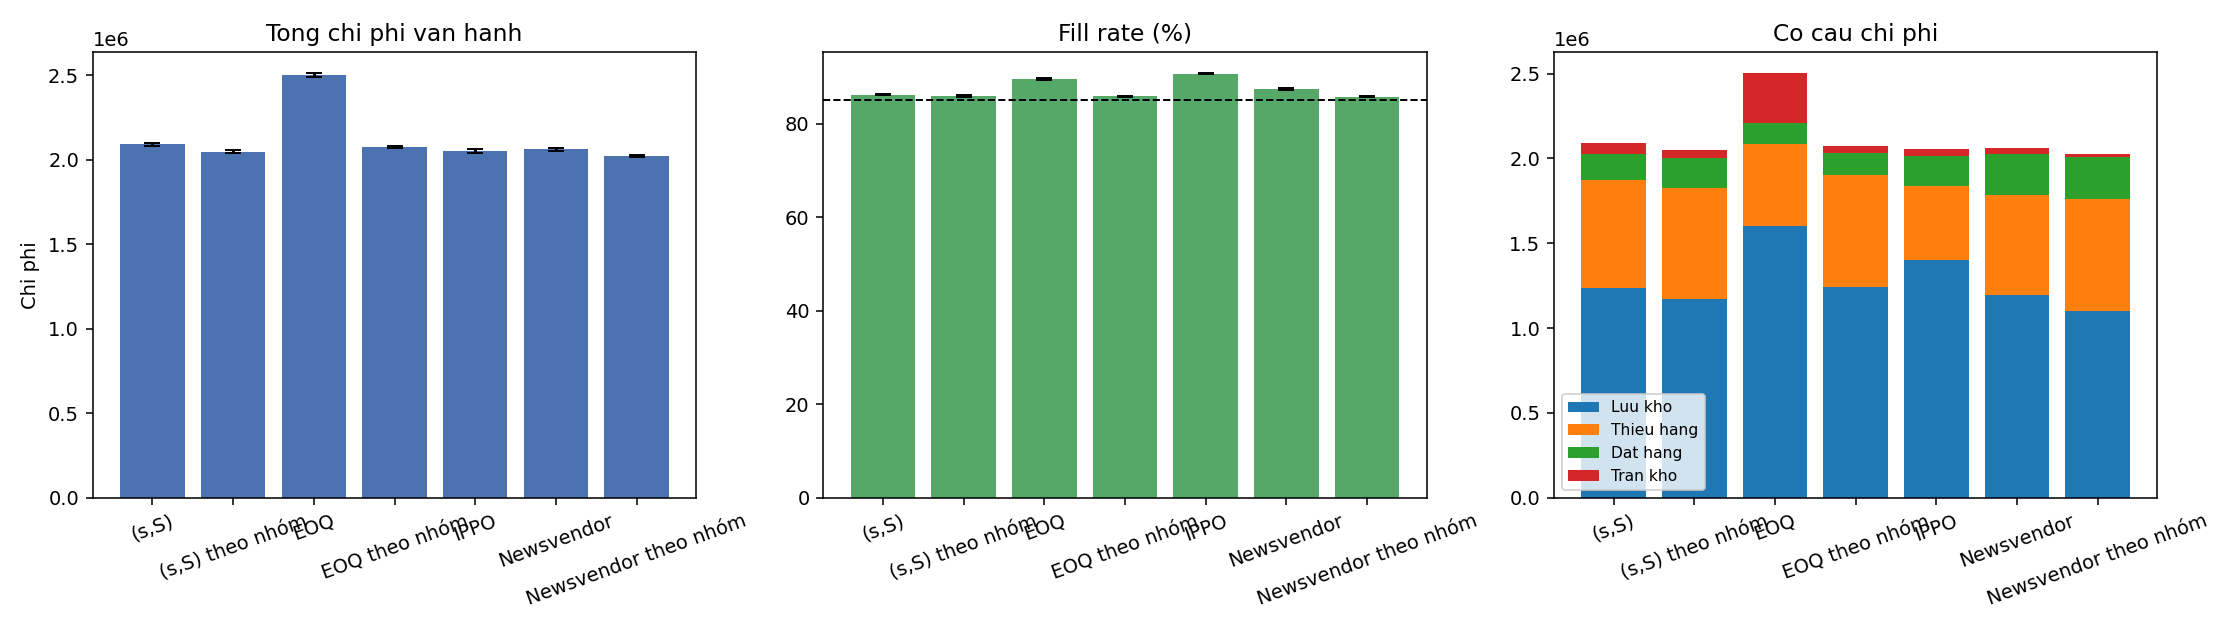
\includegraphics[width=\textwidth]{media/so_sanh_baseline.png}
    \caption{So sánh các phương pháp trên miền test (hạt giống huấn luyện $42$):
    (a) tổng chi phí vận hành; (b) tỷ lệ đáp ứng nhu cầu; (c) cơ cấu chi phí
    thành phần}
    \label{fig:soSanhBaseline}
\end{figure}

IPPO giữ mức tồn kho cao hơn --- chi phí lưu kho $1.410.006$ so với $1.233.832$
của $(s, S)$ (cao hơn $14{,}3\%$) và $1.101.764$ của Newsvendor theo nhóm (cao
hơn $28{,}0\%$) --- và dùng mức tồn kho đó để cắt giảm chi phí thiếu hàng, từ
$639.569$ xuống $420.908$ so với $(s, S)$ (giảm $34{,}2\%$) và từ $661.207$ so với
Newsvendor theo nhóm (giảm $36{,}3\%$). Với $(s, S)$, phần tiết kiệm ở thiếu hàng
lớn hơn phần tăng thêm ở lưu kho nên tổng chi phí của IPPO thấp hơn; với các
baseline theo nhóm, hai phần gần như bù nhau nên tổng chi phí xấp xỉ bằng nhau
(Newsvendor theo nhóm thậm chí rẻ hơn $1{,}6\%$). Đây đúng là chiến lược ``tích
trữ nhiều hơn để giảm thiếu hàng'' mà thành phần phạt mức phục vụ
(Mục~\ref{subsec:fillRate}) khuyến khích: tác tử được thưởng vì mức phục vụ cao
chứ không phải vì chi phí thấp nhất tuyệt đối.

Chiến lược này vẫn khả thi vì tác tử biết được giới hạn của mình. Chi phí tràn
kho của IPPO là $46.388$, tức khoảng $2{,}3\%$ tổng chi phí --- thấp hơn $(s, S)$
($3{,}2\%$) và thấp hơn nhiều so với EOQ ($11{,}7\%$), nhưng cao hơn Newsvendor
($34.491$) và Newsvendor theo nhóm ($15.743$). Điều này cho thấy tác tử duy trì
mức tồn kho sát trần sức chứa mà không vượt qua một cách mất kiểm soát. Cần thận
trọng khi gán điều này cho cơ chế phối hợp gián tiếp ở Mục~\ref{subsec:phoiHop}:
nó nhất quán với việc tác tử dùng tín hiệu $u_t^{(w(i))}$ trong vector quan sát,
nhưng phân tích tầm quan trọng đặc trưng ở Mục~\ref{subsec:kiemTraStateReward} cho
thấy chính sách đã học dựa rất ít vào tín hiệu cấp kho khi suy luận; khác biệt
nằm ở chỗ thí nghiệm bỏ hẳn tín hiệu này khi huấn luyện (Mục~\ref{subsec:ablationKhac})
làm chi phí tăng hơn gấp đôi và huấn luyện không ổn định.

Về tần suất đặt hàng, IPPO phát trung bình $35.628$ đơn trên một episode, nhiều
hơn $(s, S)$ ($30.367$ đơn), ngang $(s, S)$ theo nhóm ($35.240$) và ít hơn đáng kể
Newsvendor ($48.825$); EOQ phát ít đơn nhất ($24.248$). Như vậy mức phục vụ cao
hơn của IPPO không đến từ việc đặt hàng ít hơn mà cũng không đến từ việc đặt
dồn dập hơn các baseline mạnh nhất; nó đến từ việc giữ mức tồn kho đệm cao hơn,
đúng với cơ cấu chi phí nêu trên.

\subsection{So sánh ở cùng mức phục vụ}
\label{subsec:isoService}

So sánh tổng chi phí giữa hai chính sách có mức phục vụ khác nhau là một phép
so sánh không đầy đủ --- đây chính xác là hạn chế của phép so sánh trực tiếp ở
Mục~\ref{subsec:soSanhChiPhi}. IPPO chịu hình phạt khi fill rate xuống dưới
ngưỡng $\tau$ nên dịch chuyển tới mức phục vụ $90{,}65\%$ (hạt giống $42$, dùng
làm đại diện cho phân tích này), trong khi các chính sách đối chứng được tìm kiếm
lưới với mục tiêu tối thiểu chi phí nên dừng lại ở $85{,}8$--$89{,}5\%$. Các
phương pháp vì vậy nằm ở những điểm khác nhau trên đường đánh đổi chi phí --- mức
phục vụ, và bảng so sánh trực tiếp không kiểm soát yếu tố này nên chưa đủ căn cứ
để kết luận phương pháp nào ưu việt hơn.

Để loại bỏ yếu tố này, khóa luận thực hiện thêm một so sánh ở cùng mức phục vụ:
với mỗi chính sách đối chứng, tìm kiếm lưới được lặp lại với ràng buộc fill rate
$\ge 90{,}15\%$ (bằng mức của IPPO trừ sai số cho phép $0{,}5$ điểm phần trăm),
chọn cấu hình rẻ nhất trong số các cấu hình thỏa mãn, rồi đánh giá lại trên miền
test.

\begin{table}[htbp]
    \centering
    \caption{So sánh ở cùng mức phục vụ: cấu hình rẻ nhất của mỗi chính sách
    đối chứng đạt fill rate $\ge 90{,}15\%$ (hạt giống $42$). Cột cuối: chênh
    lệch chi phí của IPPO so với baseline (âm là IPPO rẻ hơn).}
    \label{tab:isoService}
    \begin{tabular}{|l|c|c|c|l|}
        \hline
        \textbf{Phương pháp} & \textbf{Tổng chi phí} & \textbf{Fill rate} &
        \textbf{$\Delta$ IPPO} & \textbf{Cấu hình} \\
        \hline
        IPPO & $2.052.496$ & $90{,}65\%$ & --- & --- \\ \hline
        $(s, S)$ & $2.762.256$ & $92{,}65\%$ & $-25{,}7\%$ &
        $\alpha = 0{,}90$; $q_f = 0{,}5$; $L = 4{,}0$ \\ \hline
        Newsvendor & $2.481.517$ & $92{,}28\%$ & $-17{,}3\%$ &
        $CR = 0{,}90$; $L = 4{,}0$ \\ \hline
        EOQ & \multicolumn{4}{c|}{không cấu hình nào đạt được mức phục vụ này} \\
        \hline
    \end{tabular}
\end{table}

Kết quả ở Bảng~\ref{tab:isoService} cho thấy khi buộc phải đạt mức phục vụ cao
cỡ IPPO, chi phí của $(s, S)$ tăng từ $2{,}09$ triệu (Bảng~\ref{tab:ketQuaChiPhi})
lên $2{,}76$ triệu, và của Newsvendor từ $2{,}06$ lên $2{,}48$ triệu; IPPO không
cần thay đổi gì vì mức phục vụ $90{,}65\%$ vốn là điểm vận hành nó tự chọn. Ở cùng
mức phục vụ, IPPO rẻ hơn $(s, S)$ $25{,}7\%$ và Newsvendor $17{,}3\%$. Riêng EOQ
không có cấu hình nào trong lưới tìm kiếm đạt mức phục vụ này --- do cấu trúc
lượng đặt hàng cố định không cho phép phản ứng với biến động nhu cầu.

\textbf{Cần đọc các con số này với một cảnh báo.} Lưới tham số của baseline thô
nên cấu hình được chọn vượt mục tiêu phục vụ: $(s, S)$ đạt $92{,}65\%$ và
Newsvendor $92{,}28\%$, cao hơn IPPO $2{,}0$ và $1{,}6$ điểm phần trăm và cao hơn
ngưỡng $90{,}15\%$ hơn một điểm. Phần chi phí tăng thêm do nâng mức phục vụ vượt
mức cần thiết bị tính vào khoảng cách này, nên mức $-25{,}7\%$ và $-17{,}3\%$ là
\emph{cận trên} của lợi thế chi phí của IPPO chứ không phải ước lượng chính xác;
một lưới mịn hơn quanh ngưỡng $90{,}15\%$ sẽ thu hẹp khoảng cách này. Phát biểu
chắc chắn hơn là: để lên tới mức phục vụ $\approx 90\%$, các baseline phải trả một
khoản chi phí lớn hơn IPPO một cách rõ rệt, trong khi ở mức $85$--$86\%$ chúng
ngang IPPO về chi phí (Mục~\ref{subsec:soSanhChiPhi}). Kết luận về việc phương
pháp nào ``tốt hơn'' vì thế phụ thuộc căn bản vào việc có kiểm soát mức phục vụ
hay không, và khóa luận coi phép so sánh ở cùng mức phục vụ --- kèm cảnh báo trên
--- là căn cứ phù hợp hơn để trả lời Câu hỏi nghiên cứu 1, vì nó loại bỏ được sai
lệch do các phương pháp tối ưu cho hai mục tiêu khác nhau
(Mục~\ref{subsec:phamvitrong}).

Hình~\ref{fig:danhDoi} biểu diễn trực quan cả hai phép so sánh trên cùng một
mặt phẳng chi phí --- mức phục vụ.

\begin{figure}[htbp]
    \centering
    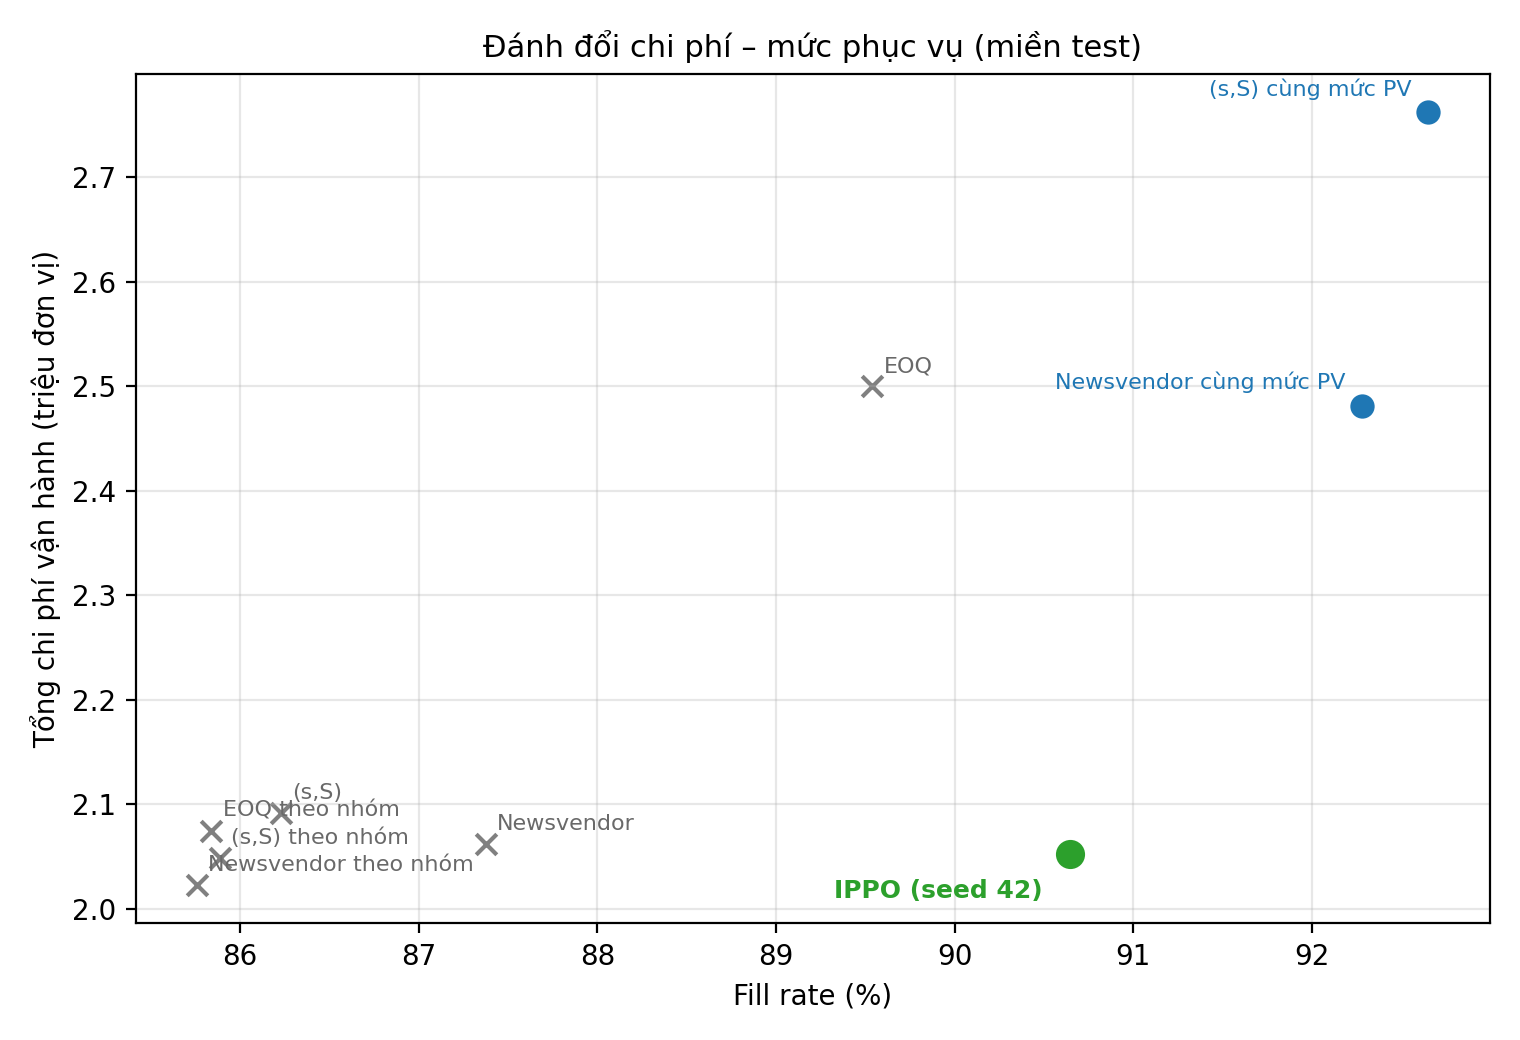
\includegraphics[width=0.72\textwidth]{media/danh_doi_chi_phi_dich_vu.png}
    \caption{Đường đánh đổi chi phí --- mức phục vụ (hạt giống $42$). Dấu chữ
    thập xám: cấu hình tối thiểu chi phí của các baseline; dấu tròn xanh dương:
    baseline chỉnh cùng mức phục vụ; chấm xanh lá: IPPO}
    \label{fig:danhDoi}
\end{figure}

Nguyên nhân của khoảng cách này nằm ở cơ chế điều chỉnh của các chính sách cổ điển.
Chúng chỉ có một cơ chế duy nhất để nâng mức phục vụ: nâng tham số an toàn ---
tăng $\alpha$ hoặc $CR$ --- và tham số đó áp dụng đồng loạt cho cả $300$ cặp. Hệ quả
là tồn kho tăng ở mọi mặt hàng, kể cả những mặt hàng vốn đã đạt mức phục vụ tốt.
IPPO điều chỉnh theo từng trạng thái quan sát được, do đó có thể nâng mức phục vụ ở những cặp có nhu cầu cấp thiết mà không tích trữ thừa ở những cặp không cần.

\section{Phân tích chuyên sâu}
\label{sec:phanTich}

\subsection{Hiệu năng theo nhóm quy mô nhu cầu (Câu hỏi 2)}
\label{subsec:tongQuatHoa}

Một bộ trọng số duy nhất điều khiển đồng thời $300$ cặp có quy mô nhu cầu trải
từ dưới $0{,}1$ đến gần $143$ đơn vị mỗi ngày. Tỷ lệ đáp ứng $90{,}6\%$ ở cấp
hệ thống là một con số có trọng số theo nhu cầu, nên nó chưa cho biết
chính sách có hoạt động đồng đều trên mọi nhóm quy mô hay không. Để trả lời,
$300$ cặp được chia thành bốn nhóm theo $\bar{D}^{(i)}$ và các chỉ số được tính
riêng cho từng nhóm (Bảng~\ref{tab:theoQuyMo}, hạt giống $42$). Chi phí trong
bảng là chi phí cục bộ trung bình mỗi cặp mỗi episode --- cùng đại lượng mà tác
tử thực sự tối ưu hóa, công thức~(\ref{eq:localReward}) --- nên bao gồm cả
thành phần định hướng mức phục vụ $\phi_{dv}$, khác với chi phí vận hành thuần
túy đã báo cáo ở Bảng~\ref{tab:ketQuaChiPhi}.

\begin{table}[htbp]
    \centering
    \caption{Hiệu năng theo nhóm quy mô nhu cầu trên miền test (hạt giống
    $42$). Chi phí cục bộ (gồm thành phần định hướng mức phục vụ) tính trung
    bình cho mỗi cặp trong một episode.}
    \label{tab:theoQuyMo}
    \small
    \begin{tabular}{|l|c|c|c|c|c|}
        \hline
        \multirow{2}{*}{\textbf{Nhóm ($\bar{D}$, đv/ngày)}} &
        \multirow{2}{*}{\textbf{Số cặp}} &
        \multicolumn{2}{c|}{\textbf{Fill rate}} &
        \multicolumn{2}{c|}{\textbf{Chi phí/cặp}} \\
        \cline{3-6}
        & & \textbf{IPPO} & \textbf{$(s,S)$} & \textbf{IPPO} & \textbf{$(s,S)$} \\
        \hline
        Rất thấp ($< 0{,}5$)     & $105$ & $74{,}2\%$ & $84{,}3\%$ & $3.164$ & $2.979$ \\ \hline
        Thấp ($0{,}5$--$2$)      & $126$ & $83{,}2\%$ & $87{,}0\%$ & $4.235$ & $4.185$ \\ \hline
        Trung bình ($2$--$10$)   & $54$  & $89{,}5\%$ & $85{,}7\%$ & $9.618$ & $10.837$ \\ \hline
        Cao ($\ge 10$)           & $15$  & $95{,}8\%$ & $86{,}4\%$ & $57.542$ & $70.926$ \\
        \hline
    \end{tabular}
\end{table}

Trên hai nhóm có nhu cầu từ $2$ đơn vị mỗi ngày trở lên, IPPO đạt kết quả tốt hơn
$(s, S)$ trên \emph{cả hai} tiêu chí: fill rate cao hơn $3{,}8$ điểm phần trăm ở
nhóm trung bình và $9{,}4$ điểm ở nhóm cao, đồng thời rẻ hơn $11{,}2\%$ ở nhóm
trung bình và $18{,}9\%$ ở nhóm cao. Các cặp có nhu cầu lớn đóng góp phần lớn
tổng chi phí hệ thống, nên đây là nơi tạo ra phần lớn lợi thế chi phí của IPPO
so với $(s, S)$ ở Mục~\ref{subsec:soSanhChiPhi}.

Ngược lại, ở hai nhóm nhu cầu thấp và rất thấp, IPPO vừa đạt mức phục vụ thấp
hơn $(s, S)$ (rất thấp: $74{,}2\%$ so với $84{,}3\%$, chênh $10{,}1$ điểm; thấp:
$83{,}2\%$ so với $87{,}0\%$) vừa có chi phí cục bộ nhỉnh hơn ($6{,}2\%$ và
$1{,}2\%$). Ở cấp từng cặp, $28{,}7\%$ số cặp của IPPO có fill rate dưới $85\%$
(phân vị $10\%$ là $71{,}2\%$), trong khi $(s, S)$ cùng mức phục vụ chỉ có
$5{,}7\%$ (Mục~\ref{subsec:kiemTraStateReward}). Cả hai nhóm này đều nằm dưới
ngưỡng $85\%$ ở IPPO hoặc sát ngưỡng, nên mục tiêu mức phục vụ \emph{không} được
đáp ứng đồng đều trên mọi mặt hàng.

Diễn giải của hiện tượng này mang tính kinh tế nhiều hơn là kỹ thuật. Với một
mặt hàng bán $0{,}3$ đơn vị mỗi ngày, chi phí một lần phát đơn ($c_{dh} = 5$)
xấp xỉ chi phí thiếu hàng của gần hai ngày bán ($c_{th} \cdot \bar{D} = 3$ mỗi
ngày). Việc duy trì mức phục vụ cao cho nhóm này đòi hỏi đặt hàng thường xuyên
với lô rất nhỏ, và tổng chi phí phát sinh vượt phần tổn thất do thiếu hàng. Tác
tử --- vốn tối thiểu hóa chi phí --- có xu hướng hạ mức phục vụ ở nhóm bán chậm, điều này phù hợp với mục tiêu tối ưu hóa chi phí mà thuật toán huấn luyện theo đuổi. Nói cách khác, chênh lệch không phải là dấu hiệu chia sẻ tham số thất bại ở nhóm bán chậm, mà là hệ quả của việc hai phương pháp theo đuổi hai mục tiêu khác nhau: $(s, S)$ được tham số hóa quanh một mức phục vụ mục tiêu, còn IPPO tối thiểu hóa chi phí dưới ràng buộc mức phục vụ ở cấp hệ thống.

Hệ quả cần ghi nhận nằm ở cách định cỡ thành phần phạt mức phục vụ. Mô hình
chính dùng hình phạt chuẩn hóa (\texttt{service\_penalty\_mode: normalized},
công thức~\ref{eq:phatChuanHoa}), trong đó sau khi chia cho mẫu số chuẩn hóa mọi
cặp chịu cùng một mức phạt $\phi_{dv} \cdot \max(\tau - \text{FR}, 0)$ bất kể quy
mô nhu cầu. Cách định cỡ này giảm nhưng không loại bỏ sự thiên lệch: ở cùng ngân
sách $1.000$ episode và cùng hạt giống, tỷ lệ cặp có fill rate dưới $85\%$ là
$28{,}3\%$ với hình phạt chuẩn hóa (\texttt{abl\_ref}) so với $33{,}0\%$ với hình
phạt tỷ lệ theo nhu cầu (\texttt{abl\_reward\_cu}); mô hình chính $10.000$ episode
đạt $28{,}7\%$. Khi đó mặt hàng bán chậm vẫn là nơi chi phí đặt hàng cố định lớn
so với phần tổn thất được tránh, và fill rate hệ thống là trung bình có trọng số
theo khối lượng, nên tác tử vẫn đạt mục tiêu chung bằng cách phục vụ tốt nhóm bán
nhanh và hạ mức phục vụ ở nhóm bán chậm (Mục~\ref{subsec:kiemTraStateReward}
định lượng hiện tượng này trên phân bố fill rate của từng cặp). Nếu bài toán
nghiệp vụ yêu cầu bảo đảm mức phục vụ tối thiểu cho từng mặt hàng, cần chuyển
mục tiêu thành ràng buộc cứng ở cấp cặp (chẳng hạn nhân tử Lagrange riêng cho
từng cặp, Mục~\ref{sec:huongPhatTrien}). Đây là một hạn chế thiết kế đã xác định,
không xuất phát từ sai lệch triển khai.

\paragraph{Mặt hàng chưa gặp khi huấn luyện (hold-out).} Để kiểm tra riêng khả
năng áp dụng cho mặt hàng chưa từng xuất hiện trong huấn luyện, một mô hình được
huấn luyện chỉ trên $24$ mặt hàng ($1.000$ episode, một hạt giống) rồi đánh giá
trên $6$ mặt hàng bị giữ lại ($6 \times 10 = 60$ cặp). So với mô hình chính của
hạt giống $42$ --- đã huấn luyện trên cả $30$ mặt hàng --- chi phí của mô hình
hold-out trên $60$ cặp này là $293.002$ (fill rate $86{,}3\%$) so với $292.774$
($86{,}8\%$), chênh $+0{,}1\%$ và không có ý nghĩa thống kê ($p = 0{,}67$). Không
có dấu hiệu suy giảm khi gặp mặt hàng mới. So với baseline, IPPO trên các mặt
hàng chưa gặp rẻ hơn $(s, S)$ $6{,}2\%$ và EOQ $28{,}4\%$ nhưng đắt hơn EOQ theo
nhóm $1{,}2\%$, Newsvendor $1{,}3\%$ và Newsvendor theo nhóm $3{,}3\%$ (đều có ý
nghĩa thống kê). Có hai lưu ý: cả sáu baseline đều có fill rate dưới $85\%$ trên
tập này ($79{,}5$--$83{,}2\%$) nên so chi phí không cùng mức phục vụ; và kết quả
chỉ trên một hạt giống với $6$ mặt hàng. Phép so sánh ``chưa gặp rẻ hơn $6{,}1\%$
so với mô hình đã gặp cùng $1.000$ episode'' không nên diễn giải là mô hình học
tốt hơn từ ít dữ liệu, vì mô hình đối chiếu $1.000$ episode đơn giản là chưa hội
tụ bằng mô hình chính ($10.000$ episode).

\subsection{Thiết kế tín hiệu phần thưởng (Câu hỏi 3)}
\label{subsec:ablationReward}

\paragraph{Thiết kế.} Câu hỏi 3 được trả lời bằng hai thí nghiệm loại trừ, cùng
mạng, cùng tốc độ học, cùng ngân sách $1.000$ episode và cùng môi trường như lần
chạy tham chiếu (\texttt{abl\_ref}), và mỗi thí nghiệm được lặp lại trên $3$ hạt
giống ($42$, $1$, $2$) để so với lần tham chiếu cùng hạt giống:
\begin{itemize}
    \item \textbf{Phần thưởng toàn cục} (\texttt{reward\_mode: global}): mọi
    tác tử nhận cùng một tín hiệu là tổng phần thưởng của cả mạng lưới
    $R_t^{\text{team}}$ (công thức~\ref{eq:mucTieuDoi}), chia cho tổng mẫu số chuẩn
    hóa của các cặp để giữ cùng thang đo. Thí nghiệm này so sánh trực tiếp phần
    thưởng cục bộ với phần thưởng toàn cục.
    \item \textbf{Không chuẩn hóa theo cặp}
    (\texttt{normalize\_reward\_per\_pair: false}): phần thưởng cục bộ của mọi cặp
    được chia cho cùng một hằng số, nên cặp có nhu cầu lớn chi phối tín hiệu học.
\end{itemize}
Hai thí nghiệm trả lời hai khía cạnh khác nhau của cùng câu hỏi thiết kế phần
thưởng và không thay thế cho nhau.

\begin{table}[htbp]
    \centering
    \caption{Thiết kế phần thưởng ($1.000$ episode mỗi lần chạy): tổng chi phí
    trên miền test, fill rate và chênh lệch so với lần tham chiếu cùng hạt giống.
    Dấu $^{*}$: kiểm định theo cặp có ý nghĩa ($p < 0{,}05$).}
    \label{tab:ablationReward}
    \small
    \begin{tabular}{|l|c|c|c|c|}
        \hline
        \textbf{Lần chạy} & \textbf{Hạt giống} & \textbf{Tổng chi phí} &
        \textbf{Fill rate} & \textbf{$\Delta$ tham chiếu} \\
        \hline
        Tham chiếu & $42$ & $2.183.787$ & $91{,}4\%$ & --- \\
                   & $1$  & $2.149.861$ & $91{,}2\%$ & --- \\
                   & $2$  & $2.179.541$ & $91{,}4\%$ & --- \\ \hline
        Phần thưởng toàn cục & $42$ & $7.711.359$ & $86{,}0\%$ & $+253{,}1\%^{*}$ \\
                   & $1$  & $11.819.736$ & $81{,}3\%$ & $+449{,}8\%^{*}$ \\
                   & $2$  & $14.293.080$ & $81{,}2\%$ & $+555{,}8\%^{*}$ \\ \hline
        Không chuẩn hóa theo cặp & $42$ & $8.972.578$ & $86{,}8\%$ & $+310{,}9\%^{*}$ \\
                   & $1$  & $5.716.403$ & $87{,}7\%$ & $+165{,}9\%^{*}$ \\
                   & $2$  & $5.798.585$ & $87{,}6\%$ & $+166{,}0\%^{*}$ \\
        \hline
    \end{tabular}
\end{table}

\paragraph{Kết quả.} Cả hai biến thể đều kém hơn rõ rệt lần tham chiếu ở cả $3$
hạt giống (Bảng~\ref{tab:ablationReward}): phần thưởng toàn cục làm tổng chi phí
tăng trung bình $419{,}6\%$ và không chuẩn hóa theo cặp tăng trung bình
$214{,}3\%$, trong khi dao động chi phí giữa $3$ hạt giống của lần tham chiếu chỉ
là $1{,}6\%$. Hai hạt giống $1$ và $2$ của phần thưởng toàn cục thậm chí không
đạt fill rate $85\%$ trên miền validation, nên checkpoint của chúng chỉ là mô
hình dự phòng và chỉ có giá trị định tính. Entropy cuối huấn luyện của hai biến
thể vẫn cao ($0{,}74$ với phần thưởng toàn cục và $0{,}48$ với không chuẩn hóa,
ở hạt giống $42$, so với $0{,}19$ của tham chiếu), nghĩa là chính sách còn gần
ngẫu nhiên hơn nhiều.

Chỉ số đáng chú ý nhất là explained variance của Critic ở hạt giống $42$:
$1{,}00$ khi không chuẩn hóa và $0{,}96$ với phần thưởng toàn cục, so với $0{,}72$
của tham chiếu. Critic giải thích \emph{gần như toàn bộ} phương sai của return,
nhưng chính sách lại học kém hơn nhiều. Điều này khớp với lập luận thiết kế ở
Mục~\ref{subsec:chuanHoaThuong}: khi return của các cặp chênh nhau nhiều bậc độ
lớn, phương sai tổng bị chi phối bởi vài cặp nhu cầu lớn. Critic chỉ cần khớp tốt
các cặp đó là đạt explained variance cao, trong khi lợi thế (advantage) của đa số
cặp bán chậm gần như chỉ còn là nhiễu. Kết quả ủng hộ giả thuyết của Câu hỏi 3
rằng phần thưởng cục bộ có chuẩn hóa theo cặp là cần thiết trong cấu hình này.
Giới hạn: các lần chạy chỉ dài $1.000$ episode, và entropy còn cao cho thấy các
biến thể có thể chỉ học chậm hơn chứ chưa chắc kém hơn ở trạng thái hội tụ; khóa
luận chưa huấn luyện chúng tới $10.000$ episode.

\subsection{Vai trò của việc tách Actor và Critic}
\label{subsec:ablationTrunk}

Bằng chứng ban đầu cho quyết định tách Actor và Critic đến từ phiên bản phát
triển đầu tiên của môi trường (dùng chung thân mạng), trong đó gradient của
hàm mất mát giá trị lớn gấp khoảng $293$ lần gradient chính sách và entropy
đứng yên gần $\ln 6 = 1{,}792$ trong giai đoạn đầu (Mục~\ref{subsec:sharedNet}).
Quan sát đó đến từ một phiên bản môi trường khác nên chưa phải thí nghiệm có
kiểm soát; thí nghiệm \texttt{abl\_trunk} bổ sung điều này trên đúng cấu hình
hiện tại ($300$ cặp, $44$ chiều): Actor và Critic chung thân mạng, một optimizer,
và tắt chuẩn hóa giá trị (value normalization). Kết quả (một hạt giống, $1.000$
episode): tổng chi phí $2.471.782$, cao hơn lần tham chiếu $13{,}2\%$ (có ý nghĩa
thống kê) và cao hơn $(s,S)$ $18{,}2\%$, fill rate chỉ $85{,}7\%$, và $20\%$ episode
cuối vẫn không đạt $85\%$ trên miền validation. Mức chênh $13{,}2\%$ lớn hơn nhiều
dao động giữa hạt giống ($1{,}6\%$), nhưng thí nghiệm thay đồng thời hai thành
phần (chung thân mạng và tắt value normalization) nên chưa tách được đóng góp của
riêng việc tách hai mạng.

\subsection{Các thí nghiệm loại trừ khác}
\label{subsec:ablationKhac}

Các thí nghiệm sau chạy $1.000$ episode, một hạt giống ($42$), so với lần tham
chiếu \texttt{abl\_ref} (Bảng~\ref{tab:ablationKhac}). Vì mỗi thí nghiệm chỉ có
một hạt giống, chênh lệch nhỏ hơn dao động $1{,}6\%$ giữa hạt giống của lần tham
chiếu (Mục~\ref{subsec:ablationReward}) chưa đủ để kết luận.

\begin{table}[htbp]
    \centering
    \caption{Thí nghiệm loại trừ ($1.000$ episode, hạt giống $42$). $\Delta$ là chênh lệch
    tổng chi phí so với \texttt{abl\_ref}; $\Delta (s,S)$ là chênh lệch so với $(s,S)$ trong
    cùng môi trường. Dấu $^{*}$: có ý nghĩa thống kê; $^{\dagger}$: môi trường đánh
    giá khác tham chiếu nên đọc cột $\Delta (s,S)$.}
    \label{tab:ablationKhac}
    \small
    \resizebox{\textwidth}{!}{%
\begin{tabular}{|l|l|c|c|c|c|}
        \hline
        \textbf{Lần chạy} & \textbf{Thay đổi} & \textbf{Tổng chi phí} &
        \textbf{Fill} & \textbf{$\Delta$} & \textbf{$\Delta (s,S)$} \\
        \hline
        \texttt{abl\_ref}      & Mốc: cấu hình chính, $1.000$ ep & $2.183.787$ & $91{,}4\%$ & --- & $+4{,}4\%^{*}$ \\ \hline
        \texttt{abl\_reward\_cu} & Phạt SLA kiểu cũ & $2.129.529$ & $90{,}8\%$ & $-2{,}5\%^{*}$ & $+1{,}8\%^{*}$ \\ \hline
        \texttt{abl\_trunk}    & Chung thân, tắt value norm & $2.471.782$ & $85{,}7\%$ & $+13{,}2\%^{*}$ & $+18{,}2\%^{*}$ \\ \hline
        \texttt{abl\_nocal}    & Bỏ đặc trưng lịch & $2.149.459$ & $91{,}1\%$ & $-1{,}6\%^{*}$ & $+2{,}8\%^{*}$ \\ \hline
        \texttt{abl\_nowh}     & Bỏ tín hiệu cấp kho & $5.273.773$ & $91{,}2\%$ & $+141{,}5\%^{*}$ & $+152{,}1\%^{*}$ \\ \hline
        \texttt{abl\_event}    & Thêm đặc trưng sự kiện tới & $2.166.864$ & $90{,}9\%$ & $-0{,}8\%^{*}$ & $+3{,}6\%^{*}$ \\ \hline
        \texttt{abl\_warm}     & Warm-start lịch sử cầu & $2.064.993$ & $90{,}8\%$ & $-5{,}4\%^{*\dagger}$ & $-1{,}1\%^{*}$ \\
        \hline
    \end{tabular}}
\end{table}

Đọc kết quả một cách thận trọng. Bỏ đặc trưng lịch ($-1{,}6\%$) và thêm đặc trưng
sự kiện sắp tới ($-0{,}8\%$) đều nằm trong dao động giữa hạt giống, nên không có
bằng chứng rằng các đặc trưng lịch giúp ích --- nhất quán với việc chúng đóng góp
ít ở phân tích tầm quan trọng đặc trưng (Mục~\ref{subsec:kiemTraStateReward}), và
đặc trưng sự kiện sắp tới không khắc phục được điểm yếu mùa lễ. Phạt SLA kiểu cũ
rẻ hơn $2{,}5\%$, chỉ hơi vượt dao động giữa hạt giống ($1{,}6\%$) nên cần nhiều
hạt giống hơn để kết luận. Warm-start lịch sử cầu rẻ hơn $5{,}4\%$ nhưng môi trường đánh giá khác
nên chỉ nên đọc theo cột $\Delta (s,S)$ ($-1{,}1\%$). Kết quả nổi bật nhất là bỏ
tín hiệu cấp kho: tổng chi phí tăng $141{,}5\%$ và $20\%$ episode cuối không đạt
$85\%$ trên miền validation, tức huấn luyện không ổn định. Điều này mâu thuẫn bề
ngoài với việc xáo trộn tín hiệu này ở bước suy luận gần như không đổi chi phí
(Mục~\ref{subsec:kiemTraStateReward}); hai thí nghiệm đo hai việc khác nhau: tín
hiệu cấp kho có thể cần thiết để \emph{học} ra việc phối hợp qua sức chứa dù chính
sách đã học không còn dựa vào nó khi vận hành. Đây là một giả thuyết cần kiểm
chứng thêm trên nhiều hạt giống.

\subsection{Thực nghiệm B: hiệu năng theo giai đoạn nhu cầu}
\label{subsec:hanChe}

Toàn bộ các kết quả ở trên (gọi chung là \emph{thực nghiệm A}) lấy trung bình
trên cả episode $365$ ngày. Trung bình dài hạn có thể che khuất một câu hỏi
quan trọng: chính sách cổ điển có tốt hơn khi nhu cầu ổn định, và học tăng
cường có lợi thế rõ hơn khi nhu cầu thay đổi nhanh hay không? Thực nghiệm B tách
kết quả theo loại ngày, không huấn luyện lại, chỉ đánh giá chính sách đã có trên
miền test (\texttt{scripts/regime\_analysis.py}).

\paragraph{Thiết kế.} Ngày trong miền test được gán nhãn theo hai cách:
\begin{itemize}
    \item \textbf{Mức biến động}: với mỗi ngày $t$ và mỗi kho $w$, tính độ lệch
    $\bigl|D_t^{(w)} / \overline{D}_{28}^{(w)} - 1\bigr|$ giữa tổng nhu cầu của
    kho và trung bình $28$ ngày trước đó, rồi lấy trung bình trên $10$ kho.
    Chia tam phân vị: \emph{ổn định} ($\le 20{,}3\%$), \emph{trung bình},
    \emph{biến động} ($> 30{,}8\%$), mỗi nhóm khoảng $164$ ngày.
    \item \textbf{Lịch}: ngày có sự kiện ($43$ ngày), ngày SNAP ($240$), cuối tuần
    ($141$), mùa lễ tháng $11$--$12$ ($61$) và ngày thường (không sự kiện, không
    SNAP, không cuối tuần; $164$ ngày).
\end{itemize}
Ngoài giai đoạn tự nhiên, thực nghiệm còn tạo \textbf{sốc cầu nhân tạo}: nhân
toàn bộ nhu cầu của $28$ ngày (ngày $1650$--$1677$) với $1{,}5$ (tăng đột biến)
hoặc $0{,}5$ (sụt giảm), rồi đo fill rate và chi phí trong $28$ ngày trước, trong
và sau cú sốc. Mỗi cấu hình chạy $30$ episode với cùng $30$ hạt giống. Bên cạnh
sáu baseline tinh chỉnh trực tiếp, thực nghiệm dùng thêm hai baseline đã chỉnh
về \emph{cùng mức phục vụ} với IPPO (Bảng~\ref{tab:isoService}), vì chỉ khi fill
rate tương đương thì so sánh chi phí mới công bằng.

Thực nghiệm B và Mục~\ref{subsec:kiemTraStateReward} dùng checkpoint của hạt
giống $42$ ($10.000$ episode), cùng checkpoint với các phân tích ở
Mục~\ref{subsec:soSanhChiPhi}--\ref{subsec:isoService}.

\begin{table}[htbp]
    \centering
    \caption{Thực nghiệm B1: fill rate và chi phí vận hành trung bình mỗi ngày
    theo giai đoạn nhu cầu ($30$ episode, miền test). Cột cuối là chênh lệch chi
    phí của IPPO so với $(s,S)$ cùng mức phục vụ (âm là IPPO rẻ hơn).}
    \label{tab:theoGiaiDoan}
    \small
    \begin{tabular}{|l|c|c|c|c|c|c|c|}
        \hline
        \multirow{2}{*}{\textbf{Giai đoạn}} &
        \multicolumn{2}{c|}{\textbf{IPPO}} &
        \multicolumn{2}{c|}{\textbf{$(s,S)$ trực tiếp}} &
        \multicolumn{2}{c|}{\textbf{$(s,S)$ cùng mức PV}} &
        \multirow{2}{*}{\textbf{Chênh}} \\
        \cline{2-7}
        & Fill & CP/ngày & Fill & CP/ngày & Fill & CP/ngày & \\
        \hline
        Ổn định        & $91{,}6\%$ & $3.874$ & $89{,}2\%$ & $3.896$ & $94{,}3\%$ & $5.475$ & $-29{,}2\%$ \\ \hline
        Trung bình     & $90{,}9\%$ & $3.981$ & $86{,}8\%$ & $4.117$ & $93{,}2\%$ & $5.502$ & $-27{,}6\%$ \\ \hline
        Biến động      & $89{,}4\%$ & $4.684$ & $82{,}7\%$ & $4.767$ & $90{,}5\%$ & $5.899$ & $-20{,}6\%$ \\ \hline
        Ngày có sự kiện & $88{,}9\%$ & $4.439$ & $80{,}6\%$ & $4.801$ & $89{,}5\%$ & $5.738$ & $-22{,}6\%$ \\ \hline
        Ngày SNAP      & $90{,}4\%$ & $4.278$ & $86{,}1\%$ & $4.329$ & $92{,}6\%$ & $5.706$ & $-25{,}0\%$ \\ \hline
        Cuối tuần      & $90{,}5\%$ & $4.408$ & $81{,}8\%$ & $4.824$ & $90{,}9\%$ & $5.567$ & $-20{,}8\%$ \\ \hline
        Mùa lễ (T11--12) & $88{,}3\%$ & $5.057$ & $84{,}7\%$ & $4.676$ & $90{,}4\%$ & $6.332$ & $-20{,}1\%$ \\ \hline
        Ngày thường    & $91{,}1\%$ & $3.962$ & $89{,}0\%$ & $3.943$ & $94{,}0\%$ & $5.540$ & $-28{,}5\%$ \\ \hline
        Toàn miền test & $90{,}6\%$ & $4.180$ & $86{,}2\%$ & $4.260$ & $92{,}7\%$ & $5.626$ & $-25{,}7\%$ \\
        \hline
    \end{tabular}
\end{table}

\begin{figure}[htbp]
    \centering
    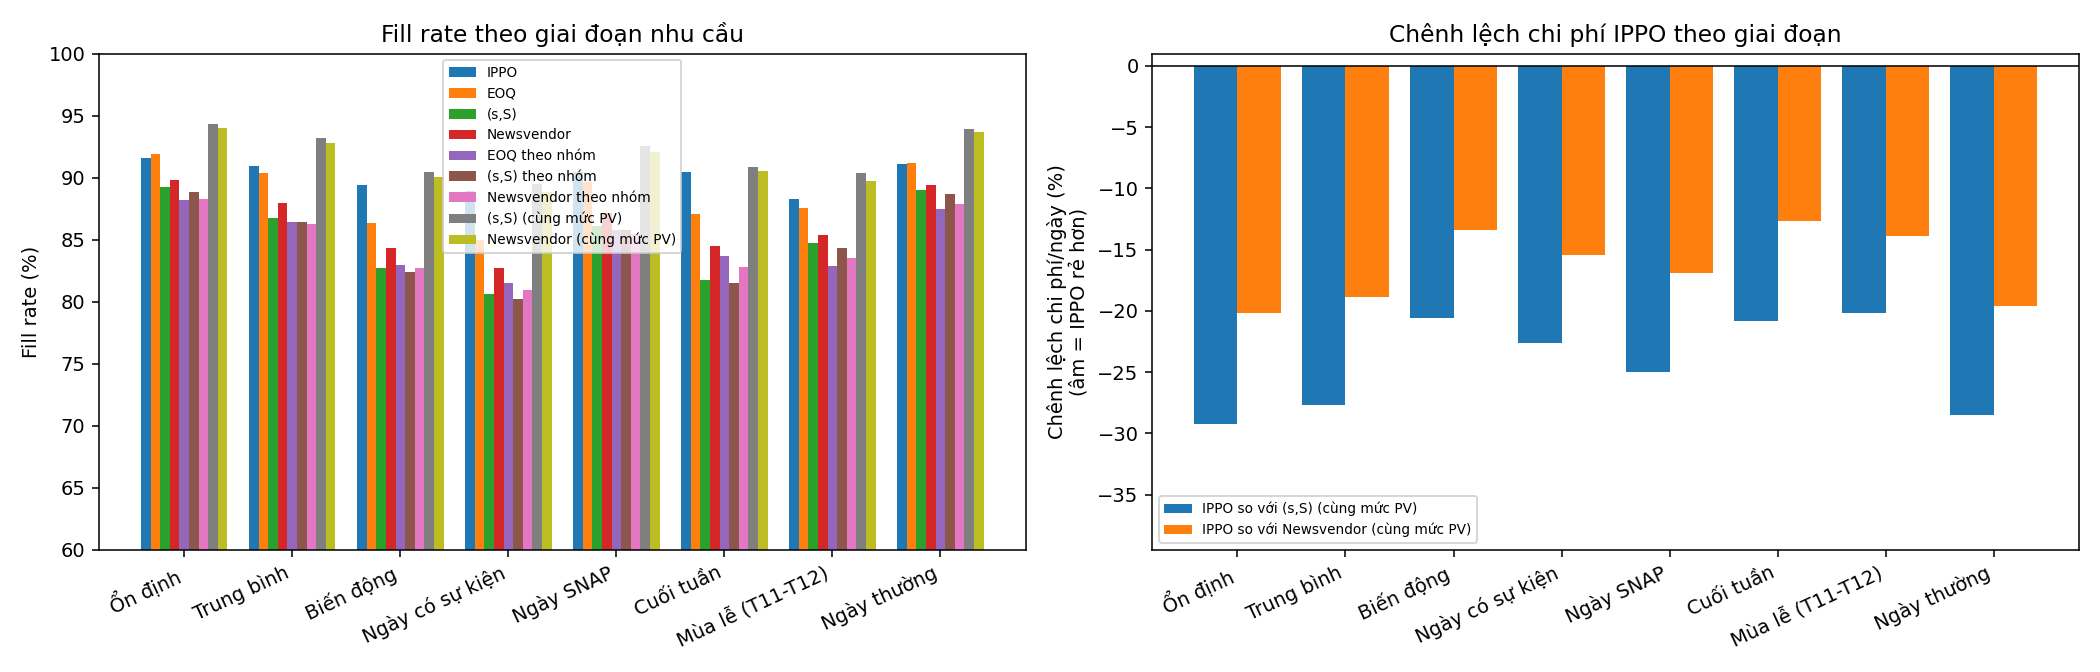
\includegraphics[width=\textwidth]{media/hinh_theo_giai_doan_nhu_cau.png}
    \caption{Thực nghiệm B1: (a) fill rate của các chính sách theo giai đoạn nhu
    cầu; (b) chênh lệch chi phí mỗi ngày của IPPO so với hai baseline ở cùng mức
    phục vụ}
    \label{fig:theoGiaiDoan}
\end{figure}

\paragraph{Kết quả B1 --- giai đoạn tự nhiên.} Bảng~\ref{tab:theoGiaiDoan} và
Hình~\ref{fig:theoGiaiDoan} cho ba nhận xét. Vì các ngày gần nhau không độc lập
(các episode chồng lấn và nhu cầu có tự tương quan), độ tin cậy của từng chênh
lệch được ước lượng bằng \emph{bootstrap theo khối $7$ ngày}: lấy mẫu lại
nguyên từng tuần ($2.000$ lần) thay vì từng ngày riêng lẻ, rồi lấy khoảng tin
cậy $95\%$ của chênh lệch chi phí (Bảng~\ref{tab:ciGiaiDoan}). Bảng này so IPPO
với ba đối thủ: $(s,S)$ tinh chỉnh trực tiếp, $(s,S)$ cùng mức phục vụ, và
Newsvendor theo nhóm --- baseline mạnh nhất ở phép so sánh trực tiếp
(Mục~\ref{subsec:soSanhChiPhi}).

\begin{table}[htbp]
    \centering
    \caption{Chênh lệch chi phí mỗi ngày của IPPO và khoảng tin cậy $95\%$
    (bootstrap theo khối $7$ ngày). Dấu $^{*}$: khoảng tin cậy không chứa $0$.}
    \label{tab:ciGiaiDoan}
    \small
    \resizebox{\textwidth}{!}{%
\begin{tabular}{|l|c|c|c|}
        \hline
        \textbf{Giai đoạn} & \textbf{So với $(s,S)$} & \textbf{So với $(s,S)$ cùng mức PV} & \textbf{So với Newsvendor theo nhóm} \\
        \hline
        Ổn định          & $-0{,}6\%$ $[-2{,}3;\ +1{,}3]$ & $-29{,}2\%$ $[-31{,}0;\ -27{,}4]^{*}$ & $+2{,}3\%$ $[+0{,}7;\ +4{,}0]^{*}$ \\ \hline
        Trung bình       & $-3{,}3\%$ $[-5{,}8;\ -0{,}6]^{*}$ & $-27{,}6\%$ $[-30{,}0;\ -24{,}8]^{*}$ & $+0{,}3\%$ $[-1{,}8;\ +2{,}6]$ \\ \hline
        Biến động        & $-1{,}7\%$ $[-7{,}5;\ +3{,}7]$ & $-20{,}6\%$ $[-23{,}6;\ -17{,}7]^{*}$ & $+1{,}8\%$ $[-2{,}5;\ +5{,}9]$ \\ \hline
        Ngày có sự kiện  & $-7{,}5\%$ $[-14{,}7;\ -0{,}2]^{*}$ & $-22{,}6\%$ $[-26{,}0;\ -19{,}2]^{*}$ & $-3{,}4\%$ $[-9{,}4;\ +2{,}5]$ \\ \hline
        Ngày SNAP        & $-1{,}2\%$ $[-4{,}6;\ +2{,}5]$ & $-25{,}0\%$ $[-27{,}5;\ -22{,}3]^{*}$ & $+1{,}5\%$ $[-1{,}0;\ +4{,}1]$ \\ \hline
        Cuối tuần        & $-8{,}6\%$ $[-12{,}9;\ -4{,}0]^{*}$ & $-20{,}8\%$ $[-23{,}1;\ -18{,}6]^{*}$ & $-2{,}6\%$ $[-6{,}2;\ +1{,}1]$ \\ \hline
        Mùa lễ (T11--12) & $+8{,}2\%$ $[-3{,}3;\ +17{,}8]$ & $-20{,}1\%$ $[-28{,}1;\ -12{,}7]^{*}$ & $+10{,}1\%$ $[+2{,}5;\ +16{,}2]^{*}$ \\ \hline
        Ngày thường      & $+0{,}5\%$ $[-2{,}9;\ +3{,}8]$ & $-28{,}5\%$ $[-31{,}3;\ -25{,}2]^{*}$ & $+3{,}3\%$ $[+1{,}0;\ +5{,}7]^{*}$ \\
        \hline
    \end{tabular}}
\end{table}

Thứ nhất, \textbf{khi nhu cầu ổn định, chính sách cổ điển cạnh tranh được, thậm
chí tốt hơn về chi phí}. Ở nhóm ngày ổn định và ngày thường, IPPO ngang $(s,S)$
tinh chỉnh trực tiếp ($-0{,}6\%$ và $+0{,}5\%$, đều không có ý nghĩa thống kê, đổi
lại fill rate cao hơn khoảng $2$ điểm phần trăm), nhưng đắt hơn Newsvendor theo
nhóm $2{,}3\%$ và $3{,}3\%$ (có ý nghĩa thống kê); ngoài ra IPPO cũng đắt hơn
$(s,S)$ theo nhóm $1{,}8\%$ ở ngày ổn định. Đây đúng là điều lý thuyết dự đoán:
khi nhu cầu gần với trung bình trượt, công thức $s = \mu_L + z\sigma_L$ là một
xấp xỉ tốt, và chính sách cổ điển được chỉnh theo nhóm không cần gì hơn.

Thứ hai, \textbf{khi nhu cầu biến động, ưu thế của IPPO thể hiện rõ ở độ bền của
mức phục vụ và ở ngày có tính chu kỳ}. Từ nhóm ổn định sang nhóm biến động, fill
rate của IPPO giảm $2{,}2$ điểm phần trăm ($91{,}6\% \to 89{,}4\%$), trong khi
$(s,S)$ trực tiếp giảm $6{,}5$ điểm ($89{,}2\% \to 82{,}7\%$) và $(s,S)$ cùng mức
phục vụ giảm $3{,}8$ điểm. Ở ngày có sự kiện và cuối tuần, IPPO vừa rẻ hơn $(s,S)$
trực tiếp ($7{,}5\%$ và $8{,}6\%$, cả hai có ý nghĩa thống kê) vừa có fill rate
cao hơn khoảng $8$--$9$ điểm --- tức ưu thế trên cả hai tiêu chí ở nhóm ngày này.
Tuy nhiên, so với Newsvendor theo nhóm, chênh lệch ở các ngày đó ($-3{,}4\%$ và
$-2{,}6\%$) không có ý nghĩa thống kê; riêng cuối tuần IPPO còn rẻ hơn có ý nghĩa
thống kê so với $(s,S)$ theo nhóm ($-7{,}2\%$) và EOQ theo nhóm ($-3{,}6\%$). Ở nhóm
``biến động'' theo độ lệch nhu cầu, chênh lệch chi phí so với $(s,S)$ trực tiếp
($-1{,}7\%$) chưa có ý nghĩa thống kê; ưu thế ở nhóm này thể hiện chủ yếu qua mức
phục vụ.

Thứ ba, \textbf{ở cùng mức phục vụ, IPPO rẻ hơn trong mọi giai đoạn}
($20{,}1\%$--$29{,}2\%$ so với $(s,S)$, $12{,}7\%$--$20{,}1\%$ so với Newsvendor,
đều có ý nghĩa thống kê). Con số này cần đọc cùng cảnh báo ở
Mục~\ref{subsec:isoService}: hai baseline cùng mức phục vụ giữ fill rate cao hơn
IPPO ở hầu hết các nhóm ngày (chẳng hạn $94{,}3\%$ so với $91{,}6\%$ ở ngày ổn
định), nên khoảng cách bị phóng đại. Ưu thế tương đối \emph{không} tăng theo mức
biến động: lớn nhất ở ngày ổn định ($-29{,}2\%$), nhỏ nhất ở nhóm biến động, cuối tuần và
mùa lễ. Mùa lễ cuối năm là giai đoạn yếu nhất của IPPO: fill rate thấp nhất
($88{,}3\%$) và chi phí mỗi ngày cao hơn $(s,S)$ trực tiếp $8{,}2\%$ (chưa có ý
nghĩa thống kê), cao hơn Newsvendor theo nhóm $10{,}1\%$ và EOQ theo nhóm $7{,}0\%$
(cả hai có ý nghĩa thống kê). Mùa lễ chỉ gồm $9$ tuần trong miền test nên khoảng
tin cậy rất rộng; nó nên được xem là một điểm yếu cần theo dõi chứ không phải một
kết luận chắc chắn. Một nguyên nhân khả dĩ là miền huấn luyện ($1.050$ ngày đầu)
chỉ chứa khoảng ba mùa lễ, và phân tích tầm quan trọng đặc trưng
(Mục~\ref{subsec:kiemTraStateReward}) cho thấy tác tử gần như không khai thác các
đặc trưng lịch.

\begin{table}[htbp]
    \centering
    \caption{Thực nghiệm B2: fill rate (và chi phí mỗi ngày) trước, trong và sau
    sốc cầu $28$ ngày}
    \label{tab:socCau}
    \small
    \begin{tabular}{|l|c|c|c|c|c|c|}
        \hline
        \multirow{2}{*}{\textbf{Chính sách}} &
        \multicolumn{3}{c|}{\textbf{Sốc tăng $\times 1{,}5$}} &
        \multicolumn{3}{c|}{\textbf{Sốc giảm $\times 0{,}5$}} \\
        \cline{2-7}
        & Trước & Trong & Sau & Trước & Trong & Sau \\
        \hline
        IPPO & $91{,}6\%$ & $83{,}5\%$ & $\mathbf{93{,}3\%}$ & $91{,}6\%$ & $97{,}8\%$ & $\mathbf{90{,}8\%}$ \\
             & ($3.724$) & ($\mathbf{5.451}$) & ($4.150$) & ($3.724$) & ($3.354$) & ($3.865$) \\ \hline
        $(s,S)$ trực tiếp & $88{,}6\%$ & $81{,}2\%$ & $89{,}6\%$ & $88{,}6\%$ & $91{,}7\%$ & $82{,}9\%$ \\
             & ($3.925$) & ($6.552$) & ($4.253$) & ($3.925$) & ($2.680$) & ($4.291$) \\ \hline
        Newsvendor trực tiếp & $90{,}2\%$ & $83{,}7\%$ & $91{,}5\%$ & $90{,}2\%$ & $92{,}0\%$ & $83{,}4\%$ \\
             & ($3.809$) & ($6.278$) & ($4.121$) & ($3.809$) & ($2.579$) & ($4.285$) \\ \hline
        $(s,S)$ cùng mức PV & $94{,}3\%$ & $84{,}8\%$ & $92{,}2\%$ & $94{,}3\%$ & $97{,}8\%$ & $90{,}5\%$ \\
             & ($5.346$) & ($9.392$) & ($6.578$) & ($5.346$) & ($3.590$) & ($5.290$) \\ \hline
        Newsvendor cùng mức PV & $94{,}6\%$ & $86{,}1\%$ & $93{,}3\%$ & $94{,}6\%$ & $96{,}6\%$ & $89{,}2\%$ \\
             & ($4.617$) & ($8.169$) & ($5.637$) & ($4.617$) & ($3.189$) & ($4.820$) \\
        \hline
    \end{tabular}
\end{table}

\begin{figure}[htbp]
    \centering
    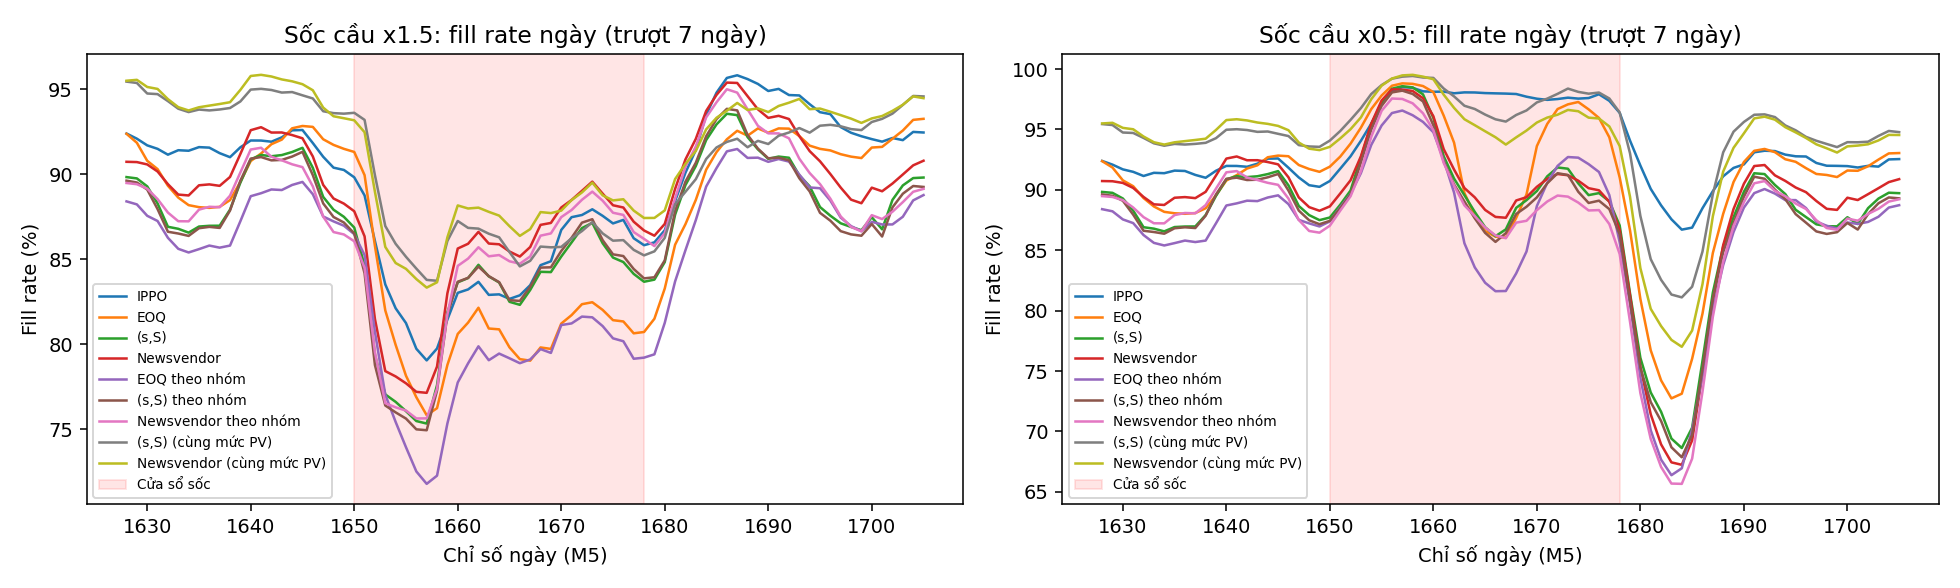
\includegraphics[width=\textwidth]{media/hinh_soc_cau.png}
    \caption{Thực nghiệm B2: fill rate theo ngày (trung bình trượt $7$ ngày)
    quanh cú sốc cầu; vùng tô đỏ là $28$ ngày bị sốc}
    \label{fig:socCau}
\end{figure}

\paragraph{Kết quả B2 --- sốc cầu.} Khi nhu cầu tăng đột ngột $50\%$
(Bảng~\ref{tab:socCau}, Hình~\ref{fig:socCau}), mọi chính sách đều mất khoảng
$6$--$10$ điểm fill rate trong cú sốc: IPPO từ $91{,}6\%$ xuống $83{,}5\%$, $(s,S)$
trực tiếp $81{,}2\%$, Newsvendor trực tiếp $83{,}7\%$. Ở mức fill rate gần như
nhau với Newsvendor trực tiếp, IPPO tốn $5.451$ đơn vị mỗi ngày so với $6.278$ của
Newsvendor ($-13{,}2\%$) và $6.552$ của $(s,S)$ ($-16{,}8\%$, kèm fill rate cao hơn
$2{,}3$ điểm). So với hai baseline cùng mức phục vụ ($9.392$ và $8.169$), IPPO rẻ
hơn $42\%$ và $33\%$ nhưng các baseline này giữ fill rate cao hơn $1{,}3$ và $2{,}6$
điểm trong cú sốc, nên khoảng cách một phần phản ánh mức phục vụ cao hơn. Sau
cú sốc, IPPO phục hồi lên fill rate $93{,}3\%$, bằng Newsvendor cùng mức phục vụ và
cao hơn các baseline còn lại.

Khi nhu cầu sụt $50\%$ rồi quay lại bình thường, khác biệt rõ hơn. Trong cú sốc
mọi chính sách đều dư hàng nên fill rate tăng. Nhưng khi nhu cầu hồi phục, các
chính sách cổ điển tinh chỉnh trực tiếp tụt mạnh ($82{,}9\%$ với $(s,S)$ và
$83{,}4\%$ với Newsvendor; đáy của fill rate trượt $7$ ngày, đọc từ Hình, khoảng
$65$--$73\%$), và hai baseline cùng mức phục vụ xuống $90{,}5\%$ và $89{,}2\%$ (đáy
trượt khoảng $77$--$81\%$), vì ước lượng $\mu$ và $\sigma$ từ cửa sổ $7$ ngày vẫn
phản ánh giai đoạn nhu cầu thấp nên chúng đặt quá ít. IPPO giữ $90{,}8\%$ (đáy
trượt khoảng $87\%$). Cần diễn giải đúng hiện tượng này: nó \emph{không} chứng
minh IPPO ``dự đoán'' được sự hồi phục, mà cho thấy chính sách học được không phụ
thuộc hoàn toàn vào cửa sổ ngắn hạn --- nó kết hợp lịch sử $7$ ngày với đặc trưng
quy mô dài hạn $\log(1 + \bar{D}^{(i)})$, đặc trưng có tầm quan trọng cao nhất
trong phân tích ở Mục~\ref{subsec:kiemTraStateReward}. Nói cách khác, IPPO bền hơn
trước nhiễu ngắn hạn, đổi lại có thể phản ứng chậm hơn nếu thay đổi nhu cầu là
vĩnh viễn.

\paragraph{Kết luận thực nghiệm B.} Kết quả không cho thấy học tăng cường đạt chi phí thấp hơn
ở mọi giai đoạn. Khi nhu cầu ổn định hoặc vào ngày thường, các chính sách cổ điển
được tinh chỉnh tốt --- đặc biệt Newsvendor theo nhóm --- rẻ hơn IPPO vài phần
trăm, dù IPPO cho fill rate cao hơn; ở mùa lễ IPPO kém nhất. Ưu thế của IPPO tập
trung ở: (1) độ bền của mức phục vụ khi nhu cầu biến động và khi hồi phục sau
cú sụt; (2) chi phí thấp hơn $(s,S)$ và $(s,S)$ theo nhóm ở ngày có sự kiện và cuối
tuần (nhưng không có ý nghĩa thống kê so với Newsvendor theo nhóm); và (3) chi
phí thấp hơn khi chống đỡ sốc tăng cầu so với các baseline cùng mức phục vụ. Hai
giới hạn của thực nghiệm này: (1) miền test chỉ dài $491$ ngày nên các episode
$365$ ngày chồng lấn nhau --- bootstrap theo khối tuần giảm nhưng không loại bỏ
hoàn toàn ảnh hưởng của tự tương quan; (2) mùa lễ chỉ có $61$ ngày ($9$ tuần) nên
kết luận về mùa lễ còn yếu.

\subsection{Kiểm tra trạng thái và phần thưởng bằng thực nghiệm}
\label{subsec:kiemTraStateReward}

Thiết kế trạng thái (Bảng~\ref{tab:doiChieuState}) và phần thưởng
(công thức~\ref{eq:localReward}) ở Chương~\ref{chap:chapter3} mới dựa trên lập
luận. Mục này kiểm tra lại bằng thực nghiệm ba câu hỏi: chính sách có hành vi
hợp lý về nghiệp vụ không, tác tử có khai thác kẽ hở của phần thưởng không, và
trạng thái có biến dư thừa không (\texttt{scripts/policy\_behavior.py}, $10$
episode trên miền test, so với $(s,S)$ cùng mức phục vụ).

\begin{figure}[htbp]
    \centering
    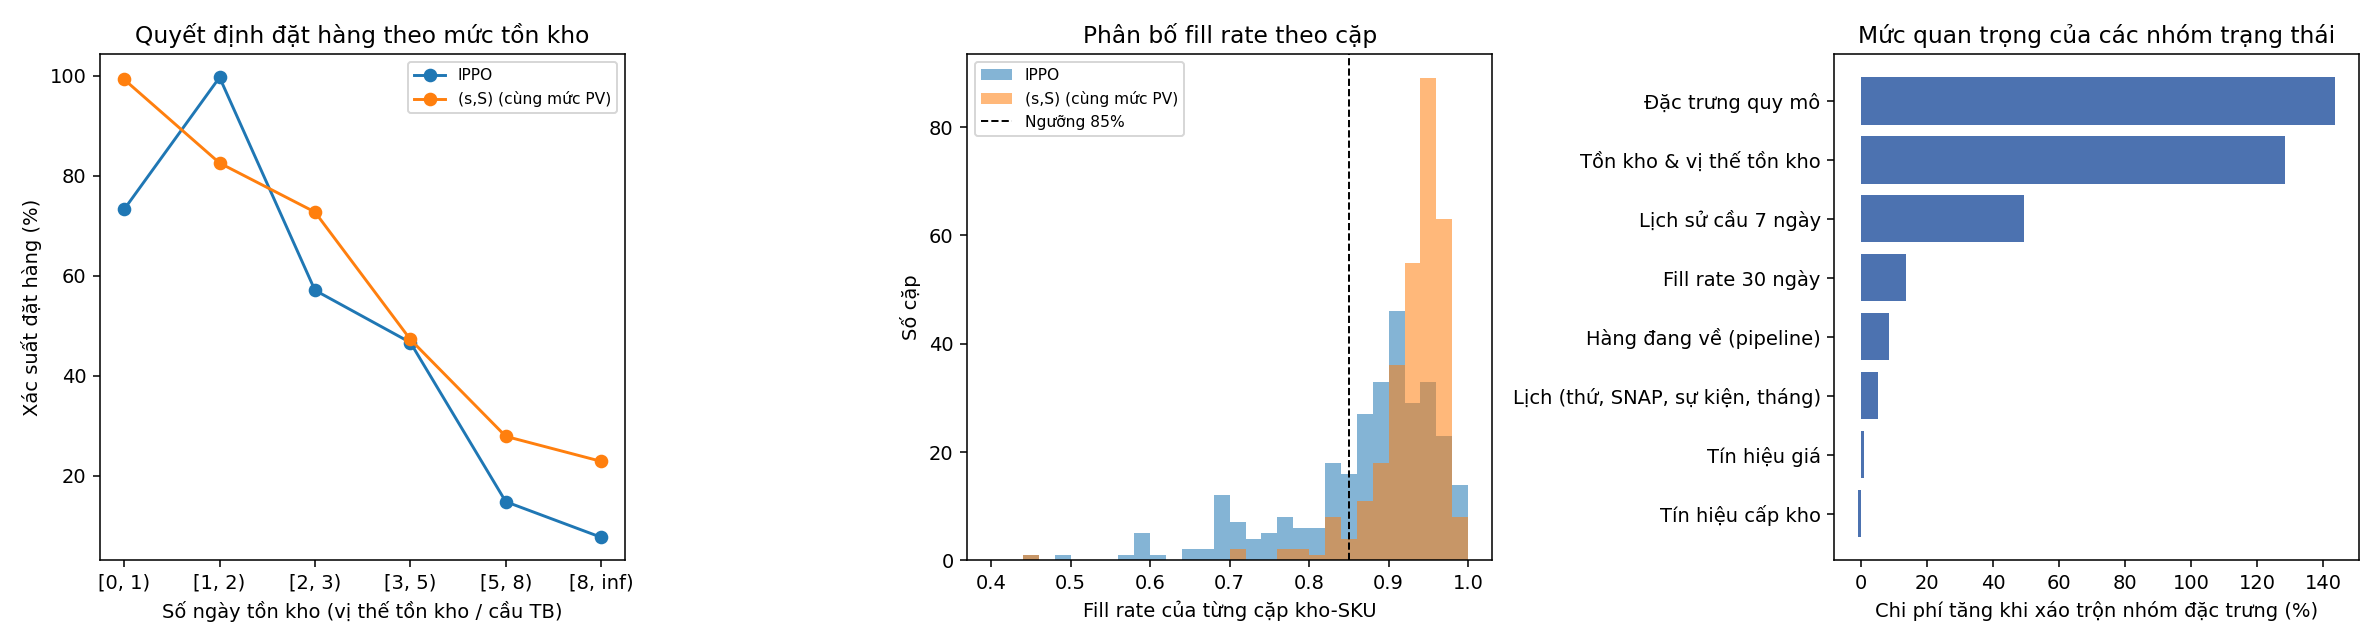
\includegraphics[width=\textwidth]{media/hinh_hanh_vi_chinh_sach.png}
    \caption{(a) Xác suất đặt hàng theo số ngày tồn kho; (b) phân bố fill rate
    của $300$ cặp; (c) mức tăng chi phí khi xáo trộn từng nhóm đặc trưng
    trạng thái}
    \label{fig:hanhVi}
\end{figure}

\paragraph{Hành vi có hợp lý về nghiệp vụ không?} Hình~\ref{fig:hanhVi}a nhóm
các quyết định theo số ngày tồn kho (vị thế tồn kho chia cho nhu cầu trung
bình). Xác suất IPPO đặt hàng giảm gần đơn điệu khi tồn kho tăng từ $2$ ngày trở
lên: $57\%$ khi còn $2$--$3$ ngày hàng, $47\%$ khi còn $3$--$5$ ngày, $15\%$ khi
còn $5$--$8$ ngày và $8\%$ khi trên $8$ ngày; khi còn $1$--$2$ ngày, IPPO đặt hàng
trong gần $100\%$ trường hợp. Tương quan hạng Spearman giữa số ngày tồn kho và
mức đặt là $-0{,}42$, mạnh hơn $(s,S)$ cùng mức phục vụ ($-0{,}17$). IPPO chỉ dùng
mức đặt lớn nhất ($5\bar{D}\bar{L}$) ở $1{,}3\%$ số quyết định, và chi phí tràn
kho chỉ chiếm $2{,}0\%$ tổng chi phí (so với $17{,}1\%$ của $(s,S)$ cùng mức phục
vụ). Có một điểm bất thường: khi tồn kho dưới $1$ ngày, IPPO chỉ đặt hàng trong
$73\%$ trường hợp, thấp hơn nhóm $1$--$2$ ngày. Khóa luận chưa kiểm tra lại với
mô hình cuối xem các trường hợp không đặt này có tập trung ở các cặp bán rất
chậm hay không; giả thuyết này nhất quán với phân tích bên dưới nhưng cần xác
minh.

\paragraph{Tác tử có khai thác kẽ hở của phần thưởng không?} Nếu tác tử chỉ
``vừa đủ'' để tránh phạt mức phục vụ, fill rate của các cặp sẽ dồn sát ngưỡng
$85\%$. Điều này không xảy ra: chỉ $12{,}0\%$ số cặp nằm trong khoảng
$[85\%, 88\%)$. Tuy nhiên, phân bố fill rate theo cặp
(Hình~\ref{fig:hanhVi}b) cho thấy một dạng khai thác khác: $28{,}7\%$ số cặp của
IPPO có fill rate dưới $85\%$ (phân vị $10\%$ là $71{,}2\%$), trong khi con số này
của $(s,S)$ cùng mức phục vụ chỉ là $5{,}7\%$ (phân vị $10\%$ là $87{,}9\%$).
Fill rate hệ thống $90{,}7\%$ của IPPO đạt được nhờ phục vụ rất tốt các mặt hàng
bán chạy, bù cho các mặt hàng bán chậm. Hình phạt chuẩn hóa giảm hiện tượng này
so với hình phạt tỷ lệ theo nhu cầu ($28{,}3\%$ so với $33{,}0\%$ cặp dưới $85\%$ ở
cùng ngân sách $1.000$ episode) nhưng không xóa bỏ nó (Mục~\ref{subsec:tongQuatHoa}):
tác tử tối ưu đúng hàm mục tiêu được giao, nhưng hàm mục tiêu đó chưa mã hóa yêu
cầu ``mọi mặt hàng đều phải đạt mức phục vụ tối thiểu''. Đây là phát hiện quan
trọng nhất của phần kiểm tra này và là lý do đề xuất ràng buộc mức phục vụ ở cấp
cặp trong hướng phát triển.

\begin{table}[htbp]
    \centering
    \caption{Tầm quan trọng của các nhóm đặc trưng trạng thái (xáo trộn nhóm
    đặc trưng giữa các cặp ở mỗi bước; riêng nhóm lịch được thay bằng lịch của
    một ngày ngẫu nhiên)}
    \label{tab:tamQuanTrong}
    \small
    \begin{tabular}{|l|c|c|c|}
        \hline
        \textbf{Nhóm đặc trưng} & \textbf{Số chiều} & \textbf{Chi phí tăng} & \textbf{Fill rate đổi} \\
        \hline
        Đặc trưng quy mô $\log(1+\bar{D})$ & $1$  & $+143{,}6\%$ & $-0{,}8$ điểm \\ \hline
        Tồn kho và vị thế tồn kho           & $2$  & $+128{,}3\%$ & $-28{,}9$ điểm \\ \hline
        Lịch sử cầu $7$ ngày                & $7$  & $+49{,}3\%$ & $-12{,}5$ điểm \\ \hline
        Fill rate cửa sổ $30$ ngày          & $1$  & $+13{,}7\%$ & $-0{,}5$ điểm \\ \hline
        Hàng đang về (pipeline)             & $3$  & $+8{,}6\%$  & $-0{,}5$ điểm \\ \hline
        Lịch (thứ, SNAP, sự kiện, tháng)    & $27$ & $+5{,}3\%$  & $-0{,}2$ điểm \\ \hline
        Tín hiệu giá (mức giảm giá)         & $1$  & $+0{,}8\%$  & $+0{,}1$ điểm \\ \hline
        Tín hiệu cấp kho (mức đầy, tỷ trọng) & $2$ & $-0{,}8\%$  & $-0{,}3$ điểm \\
        \hline
    \end{tabular}
\end{table}

\paragraph{Trạng thái có biến dư thừa không?} Bảng~\ref{tab:tamQuanTrong} đo
mức giảm hiệu năng khi phá liên hệ giữa một nhóm đặc trưng và cặp tương ứng
(permutation importance), không cần huấn luyện lại. Ba nhóm quyết định là đặc
trưng quy mô, tồn kho và lịch sử cầu; chúng tương ứng đúng với các đại lượng mà
một chính sách tồn kho cổ điển cần ($\bar{D}$, vị thế tồn kho, $\sigma$). Ngược
lại, $27$ chiều lịch chỉ đóng góp $5{,}3\%$ chi phí, còn tín hiệu giá ($1$ chiều)
và tín hiệu cấp kho ($2$ chiều) gần như không có đóng góp (xáo trộn chúng thay
đổi chi phí dưới $1\%$). Với lịch, điều này giải thích vì sao IPPO yếu nhất ở mùa
lễ (Thực nghiệm B): $27/44$ chiều quan sát gần như không được khai thác. Tín hiệu
giá --- chiều quan sát thứ $44$ được thêm vào ở đợt cuối --- cũng không được
chính sách đã học khai thác; khóa luận chưa chạy thí nghiệm loại trừ riêng cho
tín hiệu này. Với tín hiệu cấp kho, mức đóng góp nhỏ ở bước suy luận nhất quán
với việc ràng buộc sức chứa ít khi chạm ngưỡng (chi phí tràn kho $2{,}0\%$), nhưng
thí nghiệm bỏ tín hiệu này khi huấn luyện lại làm huấn luyện không ổn định
(Bảng~\ref{tab:ablationKhac}). Cần lưu ý rằng permutation importance đo mức
\emph{chính sách đã học} dựa vào một đặc trưng, không phải hiệu năng của một
chính sách được huấn luyện lại khi bỏ đặc trưng đó; thí nghiệm sau chỉ có cho
nhóm lịch và nhóm cấp kho, một hạt giống.

\subsection{Độ nhạy của kết luận theo đơn giá chi phí}
\label{subsec:doNhay}

Mọi kết luận ở trên gắn với một bộ đơn giá chi phí cụ thể
($c_{lk} = 1$, $c_{th} = 10$, $c_{dh} = 5$). Để kiểm tra kết luận có phụ thuộc
vào lựa chọn này không, mỗi chính sách được chạy một lần trên miền test
($10$ episode) và ghi lại các đại lượng vật lý: đơn vị--ngày lưu kho, đơn vị
thiếu hàng, số lần đặt, đơn vị tràn kho. Tổng chi phí sau đó được tính lại trên
lưới $3 \times 4 \times 3 = 36$ bộ đơn giá
($c_{lk} \in \{0{,}5;\ 1;\ 2\}$, $c_{th} \in \{5;\ 10;\ 20;\ 40\}$,
$c_{dh} \in \{2;\ 5;\ 10\}$; \texttt{scripts/sensitivity.py}). Các chính sách
\emph{không} được huấn luyện hay tinh chỉnh lại cho từng bộ đơn giá, nên kết quả
trả lời câu hỏi: nếu doanh nghiệp định giá chi phí khác đi thì các chính sách đã
có xếp hạng thế nào.

\begin{table}[htbp]
    \centering
    \caption{Chênh lệch tổng chi phí của IPPO theo đơn giá ($c_{dh} = 5$). Mỗi ô:
    so với $(s,S)$ trực tiếp / so với $(s,S)$ cùng mức phục vụ; âm là IPPO rẻ hơn.}
    \label{tab:doNhay}
    \small
    \begin{tabular}{|c|c|c|c|c|}
        \hline
        & $c_{th} = 5$ & $c_{th} = 10$ & $c_{th} = 20$ & $c_{th} = 40$ \\
        \hline
        $c_{lk} = 0{,}5$ & $-1{,}7\%$ / $-34{,}3\%$ & $-8{,}3\%$ / $-28{,}7\%$ & $-15{,}5\%$ / $-20{,}0\%$ & $-21{,}8\%$ / $-8{,}8\%$ \\ \hline
        $c_{lk} = 1$     & $+3{,}6\%$ / $-29{,}2\%$ & $-1{,}9\%$ / $-25{,}6\%$ & $-9{,}0\%$ / $-19{,}7\%$ & $-16{,}3\%$ / $-11{,}1\%$ \\ \hline
        $c_{lk} = 2$     & $+7{,}6\%$ / $-25{,}0\%$ & $+3{,}8\%$ / $-23{,}0\%$ & $-2{,}0\%$ / $-19{,}4\%$ & $-9{,}3\%$ / $-13{,}5\%$ \\
        \hline
    \end{tabular}
\end{table}

Hai nhận xét rút ra (Bảng~\ref{tab:doNhay}). Thứ nhất, \textbf{kết luận ở cùng
mức phục vụ nhất quán về dấu}: IPPO rẻ hơn $(s,S)$ cùng mức phục vụ ở cả $36/36$
bộ đơn giá (chênh $-8{,}1\%$ đến $-35{,}4\%$), và rẻ hơn Newsvendor cùng mức phục
vụ ở cả $36/36$ bộ (chênh $-2{,}1\%$ đến $-25{,}6\%$); nhưng như đã nêu ở
Mục~\ref{subsec:isoService}, độ lớn của khoảng cách bị phóng đại vì baseline vượt
mục tiêu phục vụ. Thứ hai, \textbf{kết luận so thẳng phụ thuộc tỷ số
$c_{th}/c_{lk}$}: IPPO rẻ hơn $(s,S)$ tinh chỉnh trực tiếp ở $26/36$ bộ đơn giá
(chênh $-22{,}8\%$ đến $+8{,}1\%$), rẻ hơn Newsvendor ở $24/36$ bộ ($-18{,}3\%$
đến $+10{,}8\%$), và với các baseline theo nhóm chỉ rẻ hơn ở $18$--$24/36$ bộ
($(s,S)$ theo nhóm $18/36$, Newsvendor theo nhóm $21/36$, EOQ theo nhóm $24/36$;
khoảng chênh rộng nhất là $-23{,}5\%$ đến $+18{,}0\%$ so với Newsvendor theo
nhóm). Trong các baseline tinh chỉnh trực tiếp, chỉ EOQ bị IPPO vượt ở cả $36/36$ bộ ($-13{,}2\%$ đến
$-25{,}7\%$). Khi thiếu hàng đắt so với lưu kho, IPPO đạt chi phí thấp hơn vì nó
giữ mức phục vụ cao hơn; khi lưu kho đắt và thiếu hàng rẻ, $(s,S)$ --- vốn chấp
nhận thiếu hàng nhiều hơn --- lại rẻ hơn. Điều này nhất quán với nhận định ở
Mục~\ref{subsec:soSanhChiPhi} rằng so thẳng hai chính sách nằm ở hai điểm khác
nhau trên đường đánh đổi là không công bằng, và rằng so với các baseline tinh
chỉnh theo nhóm, IPPO không có ưu thế chi phí ổn định.

\subsection{Độ bền khi điều kiện vận hành thay đổi}
\label{subsec:doBen}

Thí nghiệm cuối kiểm tra độ bền \emph{zero-shot}: chỉ đổi môi trường đánh giá,
giữ nguyên chính sách đã học và các baseline đã tinh chỉnh ($10$ lần đánh giá mỗi
kịch bản, \texttt{scripts/robustness.py}). Chỉ những thay đổi mà chính sách đã học
vẫn nhận làm đầu vào mới được thử: sức chứa kho, thời gian giao hàng, mức nhu cầu.

\begin{table}[htbp]
    \centering
    \caption{Độ bền zero-shot: chi phí và fill rate của IPPO, và chênh lệch chi
    phí của IPPO so với từng baseline (âm là IPPO rẻ hơn). Dấu $^{*}$: có ý nghĩa
    thống kê; $^{\sim}$: kịch bản tất định, không kiểm định được.}
    \label{tab:doBen}
    \scriptsize
    \resizebox{\textwidth}{!}{%
\begin{tabular}{|l|c|c|c|c|c|c|c|c|}
        \hline
        \textbf{Kịch bản} & \textbf{IPPO} & \textbf{Fill} & $(s,S)$ & $(s,S)$-N & EOQ & EOQ-N & NV & NV-N \\
        \hline
        Gốc                   & $2.051.839$ & $90{,}7\%$ & $-1{,}9^{*}$ & $+0{,}2$ & $-18{,}0^{*}$ & $-1{,}1^{*}$ & $-0{,}5^{*}$ & $+1{,}4^{*}$ \\ \hline
        Sức chứa $4$ ngày     & $2.191.998$ & $89{,}0\%$ & $-3{,}0^{*}$ & $+0{,}7^{*}$ & $-23{,}1^{*}$ & $+0{,}5^{*}$ & $+1{,}0^{*}$ & $+4{,}6^{*}$ \\ \hline
        Sức chứa $6$ ngày     & $2.032.325$ & $91{,}1\%$ & $-0{,}3$ & $+1{,}1^{*}$ & $-14{,}3^{*}$ & $-0{,}9^{*}$ & $-0{,}3^{*}$ & $+1{,}0^{*}$ \\ \hline
        Lead time luôn $3$    & $2.156.456$ & $88{,}1\%$ & $-3{,}1^{\sim}$ & $-2{,}0^{\sim}$ & $-20{,}4^{\sim}$ & $-10{,}5^{\sim}$ & $-0{,}0^{\sim}$ & $+0{,}2^{\sim}$ \\ \hline
        Lead time $2$--$3$    & $2.100.304$ & $89{,}3\%$ & $-2{,}4^{*}$ & $-1{,}0^{*}$ & $-17{,}5^{*}$ & $-4{,}2^{*}$ & $-0{,}1$ & $+0{,}9^{*}$ \\ \hline
        Nhu cầu $+20\%$       & $2.351.070$ & $87{,}8\%$ & $-7{,}7^{*}$ & $-5{,}4^{*}$ & $-21{,}4^{*}$ & $-5{,}7^{*}$ & $-5{,}6^{*}$ & $-3{,}3^{*}$ \\ \hline
        Nhu cầu $-20\%$       & $1.826.196$ & $93{,}3\%$ & $+7{,}0^{*}$ & $+8{,}5^{*}$ & $-12{,}7^{*}$ & $+4{,}2^{*}$ & $+6{,}8^{*}$ & $+8{,}7^{*}$ \\
        \hline
    \end{tabular}}
\end{table}

Kết quả (Bảng~\ref{tab:doBen}) cho thấy chính sách đã học bền với thay đổi sức
chứa và thời gian giao hàng --- IPPO vẫn rẻ hơn $(s,S)$ và EOQ ở mọi kịch bản đó,
và ngang hoặc hơi đắt hơn các baseline theo nhóm ($+0{,}5\%$ đến $+4{,}6\%$ ở sức
chứa $4$ ngày). Khi nhu cầu tăng $20\%$, IPPO rẻ hơn tất cả sáu baseline ($-3{,}3\%$
đến $-21{,}4\%$). Điểm yếu là khi nhu cầu giảm $20\%$: IPPO đắt hơn năm trong sáu
baseline ($+4{,}2\%$ đến $+8{,}7\%$), dù fill rate đạt $93{,}3\%$; tức chính sách
tiếp tục giữ mức phục vụ cao khi không còn cần thiết. Cần nhớ các baseline vẫn
giữ tham số đã tinh chỉnh cho môi trường gốc, nên kết quả chỉ trả lời câu hỏi
``chính sách đã có chịu đựng thay đổi thế nào'' chứ không so sánh các chính sách
được chỉnh lại cho từng kịch bản.

\section{Hạn chế của thực nghiệm}
\label{sec:hanCheChuong4}

Bốn hạn chế cần được ghi nhận khi diễn giải các kết quả trên.

Thứ nhất, số hạt giống và độ dài huấn luyện của từng thí nghiệm. Mô hình chính
được huấn luyện $10.000$ episode trên $3$ hạt giống độc lập; chi phí validation
tốt nhất đi ngang ở $20\%$ episode cuối ($+0{,}2\%$ đến $+1{,}6\%$), và
checkpoint được chọn ở episode $3.775$--$5.250$, nên $10.000$ episode đủ để hội
tụ trong cấu hình này. Tuy vậy các phân tích sâu (Thực nghiệm B, so sánh cùng mức
phục vụ, kiểm tra hành vi, độ nhạy đơn giá, độ bền zero-shot) chỉ dùng checkpoint
của hạt giống $42$; chênh lệch giữa $3$ hạt giống ở kết quả chính khá hẹp (tổng
chi phí $2.042.786$--$2.071.045$, độ lệch chuẩn $14.358$) nên rủi ro phụ thuộc
một hạt giống không lớn, nhưng chưa được kiểm chứng bằng cả $3$ hạt giống cho
từng phân tích. Các thí nghiệm loại trừ $1.000$ episode khác (ngoài thiết kế phần
thưởng) và thí nghiệm hold-out chỉ có một hạt giống, và chưa được huấn luyện tới
$10.000$ episode.

Thứ hai, độ chính xác của phép so sánh ở cùng mức phục vụ. Lưới tham số của
baseline thô nên cấu hình được chọn vượt mục tiêu $90{,}15\%$ hơn một điểm phần
trăm ($92{,}65\%$ và $92{,}28\%$), làm khoảng cách chi phí ($25{,}7\%$ và
$17{,}3\%$) bị phóng đại (Mục~\ref{subsec:isoService}). Ở phép so sánh trực tiếp,
IPPO chỉ ngang các baseline theo nhóm về chi phí, nên ưu thế duy nhất không bị
nghi ngờ là mức phục vụ cao hơn khoảng $4$--$5$ điểm phần trăm.

Thứ ba, phạm vi của bộ tham số chi phí. Phân tích độ nhạy
(Mục~\ref{subsec:doNhay}) cho thấy kết luận ở cùng mức phục vụ nhất quán về dấu
trên cả $36$ bộ đơn giá, còn kết luận so thẳng phụ thuộc tỷ số $c_{th}/c_{lk}$ và
IPPO chỉ rẻ hơn các baseline theo nhóm ở $18$--$24$ trong $36$ bộ. Tuy nhiên,
phân tích này giữ nguyên các chính sách đã học; một IPPO được huấn luyện lại với
đơn giá khác có thể học được chiến lược khác.

Thứ tư, tính đại diện của dữ liệu và mức phục vụ giữa các mặt hàng. $30$ mặt hàng
được chọn theo phân tầng để trải rộng dải quy mô nhu cầu, nhưng vẫn là một tập
con nhỏ của $3.049$ mặt hàng trong bộ dữ liệu gốc, và toàn bộ dữ liệu là dữ liệu
bán lẻ của Walmart (Hoa Kỳ). Ngoài ra, $28{,}7\%$ số cặp của IPPO có fill rate
dưới $85\%$ (Mục~\ref{subsec:kiemTraStateReward}), tức mục tiêu mức phục vụ chỉ
được đáp ứng ở cấp hệ thống.

\section{Thảo luận}
\label{sec:thaoLuan}

Kết quả cho phép trả lời Câu hỏi nghiên cứu 1, nhưng câu trả lời cần được phát
biểu cẩn trọng hơn một khẳng định đơn giản. Ở điểm vận hành mà mỗi phương pháp
tự chọn (Mục~\ref{subsec:soSanhChiPhi}), IPPO đạt tổng chi phí xấp xỉ các chính
sách cổ điển tốt nhất: rẻ hơn $(s, S)$ $1{,}7\%$ và EOQ $17{,}8\%$, ngang
$(s, S)$ theo nhóm, EOQ theo nhóm và Newsvendor, và đắt hơn Newsvendor theo nhóm
$1{,}6\%$. Cái IPPO đạt thêm là mức phục vụ cao hơn khoảng $4$--$5$ điểm phần trăm
($90{,}9\%$ so với $85{,}8$--$86{,}2\%$) với cùng một mức chi phí, theo đúng thiết
kế của thành phần phạt SLA. Khi buộc các baseline đạt mức phục vụ tương đương
(Mục~\ref{subsec:isoService}), chúng đắt hơn IPPO $25{,}7\%$ ($(s, S)$) và $17{,}3\%$
(Newsvendor), còn EOQ không có cấu hình nào đạt được; nhưng do lưới tham số thô,
baseline vượt mục tiêu phục vụ hơn một điểm phần trăm nên khoảng cách này là cận
trên. Khóa luận coi phép so sánh ở cùng mức phục vụ --- kèm cảnh báo đó --- là
căn cứ phù hợp để nói rằng IPPO cho mức phục vụ cao với chi phí thấp hơn các
baseline phải nâng tham số an toàn đồng loạt, chứ không phải rằng IPPO thắng chi
phí ở mọi nơi. Tóm lại, khẳng định phù hợp với số liệu là: IPPO \emph{không đắt
hơn} các chính sách cổ điển ở mức phục vụ cao hơn, và \emph{rẻ hơn rõ rệt} khi các
chính sách cổ điển phải tăng mức phục vụ lên tương đương; ưu thế này không mang
tính Pareto tuyệt đối. Thực nghiệm theo giai đoạn nhu cầu (Mục~\ref{subsec:hanChe})
làm rõ thêm: khi nhu cầu ổn định hoặc vào mùa lễ, baseline tinh chỉnh theo nhóm
rẻ hơn hoặc ngang IPPO; ưu thế của IPPO tập trung ở độ bền của mức phục vụ khi nhu
cầu biến động, ở ngày sự kiện và cuối tuần, và khi chống đỡ sốc cầu. Kết luận này
khớp với góp ý rằng mô hình tĩnh như EOQ có thể đủ tốt khi nhu cầu ổn định, và
học tăng cường phù hợp hơn khi giá và nhu cầu biến động.

Hai nhận xét bổ sung đáng ghi nhận.

Về vai trò của ràng buộc sức chứa, thí nghiệm hiệu chỉnh $\kappa$ ở
Mục~\ref{subsec:kichBan} cho thấy khi sức chứa đủ rộng thì bài toán suy biến
thành $300$ bài toán độc lập. Nói cách khác, chính ràng buộc sức chứa dùng
chung --- chứ không phải số lượng tác tử --- mới là thứ tạo nên bản chất đa tác
tử của bài toán. Đây là yếu tố mà hai công trình gần nhất cùng bối cảnh đều
không mô hình hóa: Zhu và Wu \cite{zhu2026spatiotemporal} giả định nguồn cung
không giới hạn, còn Nam và cộng sự \cite{jeong2026alca} chỉ xét một kho duy
nhất.

Về hiệu quả tính toán, mô hình chính cần khoảng $220$--$280$ phút huấn luyện mỗi
hạt giống trên một GPU phổ thông (RTX 3050 Laptop) và không cần mô-đun dự báo nhu
cầu học sâu: tác tử học trực tiếp từ lịch sử nhu cầu thô trong vector quan sát.
Điều này tránh được sự phụ thuộc vào chất lượng của một bộ dự báo riêng biệt ---
hạn chế mà chính Zhu và Wu \cite{zhu2026spatiotemporal} nêu ra trong phần thảo
luận của họ. Khóa luận không đưa ra kết luận về việc cách làm này vượt hay kém các
phương pháp dùng dự báo, vì chưa thực hiện phép so sánh trực tiếp với chúng; các
công trình như Gijsbrechts và cộng sự \cite{gijsbrechts2022} chỉ được dùng để đặt
bối cảnh rằng học tăng cường sâu có thể cạnh tranh với các chính sách được hiệu
chỉnh kỹ trong lớp bài toán mất đơn hàng, một nhận định phù hợp với kết quả ở trên
nhưng không phải bằng chứng của khóa luận.